% !Mode:: "TeX:UTF-8"
% !TEX encoding = UTF-8 Unicode

%----------------------------------------------------------------------------------------
% Natural Language Processing: Neural Networks and Large Language Models
%
% Copyright 2021-2026
% Tong Xiao (xiaotong@mail.neu.edu.cn) and Jingbo Zhu (zhujingbo@mail.neu.edu.cn)
%----------------------------------------------------------------------------------------

%----------------------------------------------------------------------------------------
%    CONFIGURATIONS
%----------------------------------------------------------------------------------------

%\setcounter{chapter}{11}

%----------------------------------------------------------------------------------------
%	CHAPTER 12
%----------------------------------------------------------------------------------------

\chapter{Reasoning}

\thispagestyle{chapterurl} % add urls to the header

In the previous chapters, we considered LLMs for general-purpose applications, where models generate responses based on input queries. These models can naturally handle a wide variety of tasks, such as machine translation and question answering. Therefore, many NLP problems can be framed as text generation tasks and addressed using LLMs. Beyond simple text generation, a natural next step is developing models capable of deeper thought to solve more complex problems. In particular, we wish that LLMs can generate intermediate thinking steps and thus exhibit reasoning abilities.

Reasoning has long been considered one of the most challenging problems in AI. Although the NLP community has attempted to address it using methods such as parsing sentences into logical forms, these efforts mainly relied on building reasoning models based on a series of pipeline modules, which are generally prone to cascading errors. In contrast, LLMs provide a more general framework for reasoning where the thinking path can be explicitly expressed as text and so we can enable LLMs to reason during text generation. While reasoning can be viewed as an emergent ability that arises from scaling LLMs, it requires specific strategies to invoke this capability, including CoT prompting, inference-time scaling, and training LLMs to reason.

In this chapter, we will discuss methods for improving the reasoning capabilities of LLMs. We begin by introducing basic concepts related to reasoning. Next, we present techniques for developing reasoning models. Since prompting and CoT methods have been extensively discussed in the previous chapters, here we focus on two lines of research: 1) scaling inference-time compute and 2) learning to reason. Finally, we summarize the chapter with some remarks.

%----------------------------------------------------------------------------------------
% NEW SECTION
%----------------------------------------------------------------------------------------

\section{Background and Concepts}

Here we define the reasoning problem and discuss related concepts.

\subsection{What is Reasoning?}

Historically, artificial intelligence research has categorized reasoning into three primary logical forms: \textbf{deduction} (deriving specific conclusions from known premises, such as mathematical proofs), \textbf{induction} (inferring general rules or patterns from specific examples), and \textbf{abduction} (finding the most plausible explanation for a set of observations)~\cite{peirce1931:collected}. For a long time, mainstream machine learning and NLP research primarily focused on inductive tasks. For instance, classic NLP applications like text classification and named entity recognition can be viewed as inductive tasks: models are trained to generalize mapping functions from large annotated datasets.

However, with the development of LLMs, researchers are attempting to address more difficult reasoning problems, such as complex mathematics, agentic planning, and scientific discovery, which often require rigorous deductive and abductive reasoning. Modern LLM research has revealed that the standard pre-training objective (i.e., next-token prediction over massive text corpora) is powerful enough to help models internalize knowledge of language and the world, including latent reasoning capabilities. The main challenge, however, is that reasoning is not explicitly modeled during the pre-training phase. As a result, when faced with a complex problem, LLMs attempt to output the final answer directly, rather than executing a step-by-step logical derivation.

For instance, consider a simple word problem:

\begin{quote}
\textit{If John's age is twice Mary's age, and Mary will be 10 years old in 3 years, how old is John now?}
\end{quote}

A base LLM might output an incorrect guess (e.g., 20) by simply associating the keywords ``twice'' and ``10''. In contrast, a reasoning-capable LLM might explicitly generate the logical chain before answering:

\begin{quote}
\textit{Mary is currently $10 - 3 = 7$ years old. Therefore, John is $7 \times 2 = 14$ years old.}
\end{quote}

To solve complex deductive and abductive tasks using LLMs, these latent reasoning abilities must be explicitly activated, whether through prompting techniques such as CoT or through advanced post-training paradigms such as reinforcement learning.

To better understand the reasoning problem, we can view LLM capabilities using the dual-process theory in cognitive psychology: System 1 and System 2 thinking~\cite{kahneman:2011thinking}.

\begin{itemize}
\item \vspace{0.5cm} \textbf{System 1 (Intuitive Thinking):} In human cognition, System 1 operates automatically and quickly, with little or no effort. In the context of LLMs, System 1 thinking corresponds to the paradigm where a model directly outputs the final answer in a single pass. This mode is efficient and generally sufficient for inductive tasks, such as simple question answering. However, System 1 thinking is prone to logical leaps and hallucinations when confronted with complex multi-step problems.
\item \vspace{0.3cm} \textbf{System 2 (Deliberative Thinking):} This mode is slow and conscious, requiring step-by-step logical derivation. For LLMs, System 2 thinking is engaged when the model is directed to allocate additional computational resources at inference time to explicitly generate intermediate reasoning steps. By representing the thought process as text, the LLM breaks down complex tasks, verifies intermediate conclusions, and maintains a coherent logical chain before arriving at the final answer.
\end{itemize}
\vspace{0.3cm}

For LLM reasoning, the core objective is to activate the System 2 capability. To understand this, we must look beyond traditional symbolic logic. In classic AI, reasoning is often defined as the application of hard-coded logical rules over structured knowledge bases. For LLMs, however, reasoning is an intrinsic text generation process. It can be defined as the ability to generate a coherent sequence of intermediate steps to reach the final answer. In a sense, reasoning in LLMs is a mechanism to dynamically allocate more inference compute to harder problems. Ultimately, reasoning for an LLM is the capacity to encode latent System 2 thinking into a sequence of thinking steps (reasoning steps).

\subsection{Why Reasoning Matters}

Reasoning is important in NLP research because of its application to several challenging domains:

\begin{itemize}
\item \vspace{0.5cm} \textbf{Mathematics:} Solving math problems requires strict logic. A model cannot reliably solve a problem by simply associating the numbers and keywords in the question with answers seen in similar examples. Instead, it needs to apply mathematical rules step by step to derive the correct result.
\item \vspace{0.2cm} \textbf{Coding:} Writing software is much harder than simply predicting the next word. The model must generate code based on specific user requirements and strict code logic. Especially when tackling complex problems, translating abstract requirements into functional code requires step-by-step reasoning.
\item \vspace{0.2cm} \textbf{Agentic Planning:} When an LLM is used as an autonomous agent, it has to break down big, complex goals into small, actionable steps. It also needs to plan ahead and adjust its actions if things go wrong.
\item \vspace{0.2cm} \textbf{Scientific Discovery:} Helping scientists requires looking at data, coming up with new hypotheses, and testing them carefully. This relies heavily on step-by-step logical deduction and abduction.
\end{itemize}
\vspace{0.3cm}

Beyond solving harder problems, generating reasoning steps offers practical advantages. Most importantly, it makes the model interpretable. Because the model writes down its thought process as text, humans can read it and check the logic. They can even find exactly where a mistake was made. This makes the system much easier to verify and trust. In addition, reasoning step-by-step helps reduce hallucinations. Instead of making wild guesses when faced with a hard question, the model grounds its final answer in its own logical steps, which makes the output much more reliable.

\subsection{From LLMs to Reasoning Models}

Before LLMs took over, reasoning in AI was mostly about strict rules and logic. Researchers used methods like symbolic AI and semantic parsing to translate human language into intended forms, such as knowledge graphs or database queries. While the logic in these classic systems was very clear and easy to track, the systems themselves were fragile. If they encountered a word they did not know, or if one small rule failed, the whole process would crash.

When LLMs arrived, the reasoning problem was reframed as a text generation task and could be better addressed using reasoning-oriented techniques. The development of reasoning models in the LLM era can be divided into three stages: directly guessing answers, being prompted to think, and finally, learning how to think.

Early language models were trained mainly to predict the next word. When asked a question, they tried to output the answer right away. This fast guessing worked well for simple questions or writing tasks. But for complex math or logic problems, it did not work well. The models often made mistakes or hallucinated because they did not have a way to pause and work through the problem step-by-step.

The first breakthrough came when researchers realized that LLMs already possessed hidden reasoning abilities: they just needed to be awakened. By simply using CoT prompting~\cite{wei-etal:2022chain} --- asking the model to ``think step by step'' --- the model was forced to write down its thought process before giving an answer. However, this method still relied heavily on human hints and did not actually teach the model the underlying rules of logic.

The bigger game-changer recently is using reinforcement learning to train models for reasoning. Instead of just teaching models to generate text, reinforcement learning methods train these models through trial and error. When a model finds the right logical path and gets the correct answer, it receives a reward. Over time, models like OpenAI's o1~\cite{openai:2024learning} and DeepSeek-R1~\cite{deepseek:2025r1} have shown impressive reasoning abilities, such as exploring different ideas, double-checking their own steps, and fixing mistakes on their own.

These self-correction and exploration abilities lead to an important research direction: inference-time scaling \cite{snell-etal:2024scaling}. The idea is straightforward: by allocating more computational power during generation, the model can think more deeply to solve harder problems. Ideally, a model would adjust its thinking time based on how difficult a problem actually is. However, many current reasoning models take a simpler approach --- they just apply a long thinking process to all queries.

Taking a broader view, scaling compute at inference time benefits reasoning in general. Even if an LLM has not been specifically trained to reason, we can still boost its problem-solving abilities by simply giving it more compute to ``think''. For example, we can ask the model to generate multiple different reasoning paths and vote on the best one, or we can use search algorithms to help it find the correct logical steps.

Reasoning models also motivate the recent development of agents based on LLMs \cite{yao-etal:2023react,wang-etal:2024survey}. For an AI agent to complete tasks on its own, it needs reasoning to figure out how to reach a goal step by step. Because real-world tasks rarely go perfectly, the agent also has to realize when it makes a mistake and know how to fix it. All of these require the agent to have good reasoning abilities.

The rapid development of reasoning models also presents interesting but challenging research directions \cite{li-etal:2025system,chen-etal:2026towards}. One direction focuses on efficiency. For example, if models learn to dynamically adjust their thinking time, they will not waste compute on simple questions, but will only slow down for the hard ones. Another direction is expanding reasoning beyond subjects with strict right-or-wrong answers, like math or coding, to handle open-ended real-world situations. In addition, enabling models to reason across different types of data, such as images, audio, and physical environments, is a key step toward building more advanced AI systems.

%----------------------------------------------------------------------------------------
% NEW SECTION
%----------------------------------------------------------------------------------------

\section{Reasoning via Prompting}

Prompting is the simplest method to elicit reasoning from LLMs. Because it does not require any modifications to model architectures or parameters, we can simply use well-crafted input texts to stimulate the LLM into outputting the reasoning process. One of the most widely used prompting methods is chain-of-thought (CoT) prompting. The core idea is to encourage the model to generate intermediate logical derivations before producing the final answer. This is typically achieved by providing a few step-by-step examples in the prompt, or by simply appending a direct instruction like ``Let's think step by step'' to the query. Below is an example of CoT prompting, where the CoT instruction is highlighted.

\vspace{0.5em}
\begin{tcolorbox}[frame empty]

\begingroup
\setlength{\leftskip}{2em}
\setlength{\rightskip}{2em}

Q: Tom bought 3 pairs of shoes for $\$40$ each and 2 shirts for $\$20$ each. If he uses a $10\%$ discount coupon on the entire purchase, how much does he pay in total?

\vspace{0.3em}

A: \ctext[RGB]{154, 245, 175}{Let's think step-by-step.}

\vspace{0.3em}

\uline{First, calculate the total cost of the shoes: $3$ pairs multiplied by $\$40$ equals $\$120$. Next, calculate the total cost of the shirts: $2$ shirts multiplied by $\$20$ equals $\$40$. The total cost before the discount is $\$120 + \$40 = \$160$. The discount is $10\%$ of $\$160$, which is $\$16$. Finally, subtract the discount from the total cost: $\$160 - \$16 = \$144$. So the answer is $\$144$.}

\endgroup

\end{tcolorbox}
\vspace{0.5em}

In this example, the LLM produces a reasoning path (underlined text) which contains both the reasoning process and the final answer. More formally, given a CoT prompt $\mathbf{x}$\footnote{Here a CoT prompt consists of both the user input and the CoT instruction.}, the LLM generates the most likely output by maximizing the language modeling score, like this
\begin{eqnarray}
\hat{\mathbf{y}} & = & \argmax_{\mathbf{y}} \Pr(\mathbf{y} | \mathbf{x}).
\end{eqnarray}

\noindent Here $\Pr(\mathbf{y} | \mathbf{x})$ is the text generation probability as in standard language models. Each output is a token sequence $\mathbf{y}=y_0...y_n$. It represents a reasoning path consisting of a sequence of reasoning steps:
\begin{eqnarray}
\mathbf{y} & = & \{\bar{\mathbf{y}}_1,...,\bar{\mathbf{y}}_{n_p}\}. \label{eq:reasoning-path-notation}
\end{eqnarray}

\noindent Here $n_p$ is the number of reasoning steps. Each step $\bar{\mathbf{y}}_i$ is a sub-sequence of $\mathbf{y}$, which represents a single logical deduction or intermediate calculation. Note that there are many strategies to divide a reasoning path into discrete steps, such as segmenting by individual mathematical operations. For simplicity, in this example, we treat each sentence as an individual reasoning step. Hence, we have

\[
\begin{array}{rl}
\bar{\mathbf{y}}_1: & \text{First, calculate the total cost of the shoes: }\nonumber \\
& \text{$3$ pairs multiplied by $\$40$ equals $\$120$.} \nonumber \\
\bar{\mathbf{y}}_2: & \text{Next, calculate the total cost of the shirts: } \nonumber \\
& \text{$2$ shirts multiplied by $\$20$ equals $\$40$.} \nonumber \\
\bar{\mathbf{y}}_3: & \text{The total cost before the discount is $\$120 + \$40 = \$160$.} \nonumber \\
\bar{\mathbf{y}}_4: & \text{The discount is $10\%$ of $\$160$, which is $\$16$.} \nonumber \\
\bar{\mathbf{y}}_5: & \text{Finally, subtract the discount from the total cost: $\$160 - \$16 = \$144$.} \nonumber \\
\bar{\mathbf{y}}_6: & \text{So the answer is $\$144$.} \nonumber
\end{array}
\]

Given such a reasoning path, we can extract the answer from its last step. There are many ways to improve this simple CoT-based reasoning approach. For instance, techniques like self-consistency sample multiple reasoning paths and take a majority vote to identify the most reliable answer \cite{wang-etal:2023self}. Other strategies include problem decomposition to break complex queries into manageable sub-tasks \cite{zhou-etal:least}, self-reflection methods that prompt the model to critique and correct its own logical errors \cite{shinn-etal:2023reflexion,madaan-etal:2024self}, and deliberate reasoning frameworks that efficiently explore multiple branching reasoning paths \cite{yao-etal:2024tree}.


As various CoT-based prompting techniques have been presented previously, we will not go into detail here. Readers are encouraged to review the techniques covered in Chapter \ChapterLLMPrompting.


%----------------------------------------------------------------------------------------
% NEW SECTION
%----------------------------------------------------------------------------------------

\section{Inference-time Reasoning}
\label{sec:inference-time-reasoning}

Inference-time reasoning is closely related to scaling during inference, which has been introduced in Chapter \ChapterLLMInference. In this section, we extend the previous discussion and focus more on improving the reasoning performance of LLMs.

\subsection{Inference-Time Compute Scaling}

The success of LLMs heavily depends on scaling up computing power. A common way to improve these models is training-time scaling. By simply using more training data, larger model sizes, and more compute, researchers have built very powerful LLMs \cite{kaplan-etal:2020scaling,hoffmann-etal:2022training}.

However, just scaling up the training process is not enough for complex reasoning tasks. Unlike simple text generation, reasoning needs step-by-step logic and planning. It is impossible to show a model all possible reasoning paths during training. If we only rely on training to solve hard math or logic problems, we would need a very large amount of data. Ideally, we want the model to use simple logical steps to construct its own reasoning path on the fly. Therefore, it is more appealing to activate  such reasoning abilities during inference.

Because of this, a natural idea is to scale compute during the inference phase. Thus, the LLM can spend more time exploring different reasoning steps before giving the final answer. A clear benefit of this approach is that it allows for a much more flexible and efficient use of computing resources. For example, for complex math or logic problems, the LLM can allocate more time and power, and thus ``think'' longer. In many cases, a smaller model that is given extra time to reason during inference can even outperform a much larger model that is forced to give an immediate answer. We summarize the differences between training-time scaling and inference-time scaling in Table \ref{tab:scaling-comparison}.

\begin{table}[t]
\centering
\begingroup
\renewcommand{\arraystretch}{1.3}
\begin{tabular}{R{0.20\linewidth} | L{0.33\linewidth} | L{0.33\linewidth}}
Feature & Training-Time Scaling & Inference-Time Scaling \\
\hline
How it Works & Making the model bigger and feeding it more data during the initial learning phase. & Keeping the model size fixed, but giving it more compute to "think" (e.g., exploring different paths) before answering. \\ \hline
Cost to Train & Extremely high. Very expensive and hard to fix if something goes wrong. & Low to medium. We may pay to train smaller models to check its answers. \\ \hline
Cost to Use & Predictable. The cost to generate a token is mostly based on the model's size and the length of the context. & Flexible but can get very high. The deeper the model ``thinks'', the more expensive it gets.\\ \hline
Hardware Needs (Inference) & Needs high memory bandwidth for fast data reading and writing. & Needs the same high bandwidth, plus large memory capacity to explore multiple long reasoning paths. \\ \hline
Data Needed & Massive amounts of general text. & High-quality, step-by-step examples (like math proofs) and a clear way to score if an answer is right or wrong.
\end{tabular}
\caption{Comparison of training-time and inference-time scaling}
\label{tab:scaling-comparison}
\endgroup
\end{table}

We can view inference-time scaling as a problem of \textbf{search scaling}. When we give the model extra compute to ``think'', we are essentially allowing it to explore a larger space of possible logical steps, and to have a much higher chance of finding the optimal solution. This  leads to three key questions:

\begin{itemize}
\item \vspace{0.5em} How to generate different reasoning paths?
\item \vspace{0.3em} How to search through possible steps to find the best one?
\item \vspace{0.3em} How to check if the intermediate steps and final answers are correct?
\end{itemize}
\vspace{0.5em}

In the next subsections, we will address these questions by discussing three topics: sampling multiple reasoning paths (Section~\ref{sec:sampling-reasoning-paths}), search strategies for reasoning (Section~\ref{sec:search-strategies-for-reasoning}), and verification (Section~\ref{sec:reasoning-verification}).

\subsection{Sampling Multiple Reasoning Paths}
\label{sec:sampling-reasoning-paths}

The most straightforward way to scale compute during inference is to generate not just one, but multiple reasoning paths for a single input. By generating multiple different paths, we give the LLM more chances to find the correct logic and the corresponding answer.

To achieve this, it is common practice to introduce randomness into the text generation process. A typical method is to use temperature sampling, combined with top-$k$ or nucleus (top-$p$) sampling. In standard auto-regressive generation, at each position $i$, the LLM outputs a probability distribution $\Pr(\cdot | \mathbf{x}, \mathbf{y}_{< i})$ over the vocabulary $V$ for the next token $y_i$ based on its logits $u_{y_i}$. Temperature sampling modifies this distribution by scaling the logits with a temperature parameter $T > 0$ before applying the Softmax function:
\begin{eqnarray}
\Pr(y_i | \mathbf{x}, \mathbf{y}_{< i}) & = & \frac{\exp(u_{y_i} / T)}{\sum_{y'_i \in V} \exp(u_{y'_i} / T)}.
\end{eqnarray}

\noindent A higher temperature flattens the distribution, thereby encouraging the model to explore a wider variety of reasoning steps. However, unconstrained randomness can lead to degenerate or illogical text by occasionally sampling from the ``long tail'' of low-probability tokens. To maintain the quality of the generated paths, temperature sampling is typically combined with vocabulary truncation methods:

\begin{itemize}
\item \vspace{0.5em} \textbf{Top-$k$ sampling} restricts the sampling pool to only the $k$ most likely next tokens, redistributing the probability mass among them.
\item \vspace{0.3em} \textbf{Nucleus (top-$p$) sampling} uses a dynamic truncation strategy. It selects the smallest set of top-ranked tokens whose cumulative probability exceeds a threshold $p$.
\end{itemize}
\vspace{0.5em}

By applying these stochastic decoding strategies, given an input $\mathbf{x}$, the LLM can sample a set of diverse output sequences (i.e., candidate reasoning paths):
\begin{eqnarray}
\mathcal{Y}^{\mathrm{top}} & = & \{\hat{\mathbf{y}}^1, \dots, \hat{\mathbf{y}}^N\}.
\end{eqnarray}

\noindent Here $N$ represents the inference-time compute budget. The larger $N$ is, the more compute we spend exploring different reasoning paths. Once we have this diverse set of paths, the next problem is how to select the best one. There are two widely used methods for this: Best-of-$N$ and self-consistency.

\subsubsection{Best-of-$N$ (BoN)}
We have previously introduced Best-of-$N$ sampling in Section \ChapterLLMTuning\ as a method for inference-time alignment. In that context, we used a reward model $r(\mathbf{x}, \hat{\mathbf{y}})$ to select the output that best aligns with human preferences.

For reasoning tasks, the concept of BoN sampling remains the same, but the goal shifts. Instead of a preference reward model, the ``judge'' is usually a verifier (which we can denote as a general scoring function $v$) designed to evaluate how logically sound a reasoning path is. The verifier assigns a score $v(\mathbf{x}, \hat{\mathbf{y}})$ to each sampled path, and we select the best reasoning path $\hat{\mathbf{y}}_{\mathrm{best}}$ that maximizes the score
\begin{eqnarray}
\hat{\mathbf{y}}_{\mathrm{best}} & = & \argmax_{\hat{\mathbf{y}} \in \{\hat{\mathbf{y}}^1, \dots, \hat{\mathbf{y}}^N\}} v(\mathbf{x}, \hat{\mathbf{y}}).
\end{eqnarray}

\noindent The final answer is then extracted from this highest-scoring path.  To understand the BoN process, let us consider an intuitive analogy. Imagine there is a classroom of $N$ students solving a math problem	. A teacher (the verifier) grades all their scratchpads, and then picks the student with the highest score.

While BoN sampling is powerful, its effectiveness depends on the quality of the verifier. If the verifier is weak, it can easily be fooled by flawed logic that accidentally arrives at the correct final answer (i.e., reward hacking). The design of verifiers will be discussed in more detail in Section~\ref{sec:reasoning-verification}.

\subsubsection{Self-Consistency}
An alternative approach to selecting the best path via a learned verifier is self-consistency. Self-consistency relies on the intuition that in complex reasoning tasks, there are often multiple different logical paths that lead to the same correct answer, whereas incorrect reasoning paths are likely to be diverse and lead to random errors. Instead of scoring the reasoning process, self-consistency directly marginalizes out the reasoning paths by taking a majority vote over the final answers. Formally, let $A$ be the set of all possible final answers. For each sampled path $\hat{\mathbf{y}}^k$, we extract its final predicted answer $\hat{a}^k = \mathrm{Extract}(\hat{\mathbf{y}}^k)$. The self-consistency strategy selects the answer $\hat{a}_{\mathrm{sc}}$ that appears most frequently among the $N$ sampled paths:
\begin{eqnarray}
\hat{a}_{\mathrm{sc}} & = & \argmax_{a \in A} \sum_{k=1}^N \mathbbm{1}(\mathrm{Extract}(\hat{\mathbf{y}}^k) = a),
\end{eqnarray}

\noindent where $\mathbbm{1}(\cdot)$ is the indicator function.

\subsubsection{Balancing Diversity and Quality in Sampling}

When sampling multiple reasoning paths for inference-time compute scaling, we need to seek a trade-off between diversity and quality. In reasoning tasks, we often desire a diverse set of sampled paths, which increases the chance of containing the correct logic. A common heuristic is increasing the sampling temperature. By making the distribution flatter, the sampling process avoids concentrating only on a few high-probability paths. As a result, lower-probability paths are more likely to be chosen, and the model can explore a wider variety of reasoning paths within the $N$ samples. However, as temperature increases, although the diversity of the samples improves, the average logical quality of individual paths may degrade.

To achieve a balance between diversity and quality, a straightforward method is to modify the search objective during the inference stage by introducing an explicit penalty or bonus term. In this setup, diversity can be mathematically modeled as a function that is combined with the original generation probability. More formally, the modified search objective can be written as
\begin{eqnarray}
\mathrm{score}(\mathbf{x},\mathbf{y}) & = & \log \Pr(\mathbf{y}|\mathbf{x}) + \lambda D(\mathbf{y},\mathcal{Y}^{\mathrm{top}}). \label{diversity-quality-inference}
\end{eqnarray}

\noindent Here $\log \Pr(\mathbf{y} | \mathbf{x})$ favors outputs with higher probabilities, while $D(\mathbf{y},\mathcal{Y}^{\mathrm{top}})$ serves as the penalty or bonus term that encourages diversity relative to the sampled paths $\mathcal{Y}^{\mathrm{top}}$. The hyperparameter $\lambda$ controls the strength of this trade-off.
The design of $D(\cdot)$ can be quite flexible. For example, a simple penalty might decrease the scores of tokens or $n$-grams that have already appeared frequently in $\mathcal{Y}^{\mathrm{top}}$. Conversely, a bonus function could be designed to reward distinct semantic differences. Thus, the LLM can produce new reasoning structures rather than minor rephrasings of the same idea.

From a broader perspective, this sampling dilemma is also related to the exploration--exploitation trade-off studied in reinforcement learning \cite{Sutton-and-Barto:2018RL}. In RL-based tuning, an LLM can be viewed as a policy $\pi_\theta$ that generates a reasoning path $\mathbf{y}$ for a question $\mathbf{x}$. A general regularized objective can be written as
\begin{equation}
\max_{\pi_\theta} \mathbb{E}_{\mathbf{y}\sim\pi_\theta} \left[R(\mathbf{x},\mathbf{y})\right] - \beta D_{\mathrm{KL}} \left( \pi_\theta(\cdot|\mathbf{x}) \,\|\,  \pi_{\mathrm{ref}}(\cdot|\mathbf{x}) \right) + \alpha \mathrm{Entropy} \left( \pi_\theta(\cdot|\mathbf{x}) \right),
\label{diversity-quality-rl}
\end{equation}

\noindent where $R(\mathbf{x},\mathbf{y})$ measures the quality of the generated reasoning path. The KL-divergence term constrains the learned policy to remain close to the reference policy. Its main purpose is to prevent excessive policy drift, and thus reduce undesirable behaviors such as reward hacking or degradation of language quality. By contrast, the entropy term explicitly encourages the policy to maintain a less concentrated distribution and therefore promotes exploration during training.

There is a conceptual connection between the RL objective and the diversity--quality trade-off at inference time, although the two objectives operate in different spaces. At inference time, the search procedure controls how broadly it explores reasoning paths generated by a fixed model. In RL-based tuning, the KL regularization controls how far the learned policy is allowed to move away from the reference policy. A larger KL coefficient keeps the policy close to the reference model, whereas a smaller coefficient permits the optimization process to explore a broader region of the policy space in search of higher-reward behaviors. Such policy changes may enable the model to generate reasoning paths that are unlikely under the reference policy and may therefore lead to a wider range of outputs.

Both inference-time search and KL-regularized RL involve a balance between conservative behavior and broader exploration. The difference is that inference-time methods explore different outputs under a fixed model, whereas RL searches the policy space by updating the model parameters. In either case, allowing broader exploration may discover better and more varied reasoning behaviors, but excessive exploration may reduce quality or stability.

\subsection{Search Strategies for Reasoning}
\label{sec:search-strategies-for-reasoning}

In practice, finding the optimal reasoning path can be directly cast as a classic search problem: we start from an initial state, take an action to generate a reasoning step, expand the current state into a new set of states, and repeat this process until a termination condition is met. Since we have already introduced several classic search algorithms (such as tree search and beam search) in Chapter \ChapterLLMInference, we will not revisit the details of these algorithms here. Instead, we focus on how to map the search for reasoning paths onto these classic search frameworks.

To apply a search algorithm to LLM reasoning, we need to define the standard components of a search problem:

\begin{itemize}
\item \vspace{0.5em} \textbf{Search State}: For LLM reasoning, the state is the context the model has built so far. Specifically, at step $t$, the state $s_t$ consists of the original query $\mathbf{x}$ combined with the partial reasoning path generated up to this point: $s_t = (\mathbf{x}, \bar{\mathbf{y}}_1, \dots, \bar{\mathbf{y}}_t)$.
\item \vspace{0.3em} \textbf{Action}: An action is the generation of the next reasoning step (text segment) $\bar{\mathbf{y}}_{t+1}$.
\item \vspace{0.3em} \textbf{Transition Model}: Taking an action simply appends the new text segment to the existing state. This produces the next state: $s_{t+1} = (s_t, \bar{\mathbf{y}}_{t+1}) = (\mathbf{x}, \bar{\mathbf{y}}_1, \dots, \bar{\mathbf{y}}_t, \bar{\mathbf{y}}_{t+1})$.
\item \vspace{0.3em} \textbf{State Evaluation Function}: This is a scoring function that assesses the logical correctness of the current state toward the final answer. For example, to evaluate search states, we can use hard-coded heuristics, or a trained neural verifier.
\item \vspace{0.3em} \textbf{Termination Condition}: The criteria for stopping the search. This occurs when the model explicitly generates a final answer sequence, or when the search reaches a predefined computational budget (e.g., a maximum depth of explored nodes).
\end{itemize}
\vspace{0.5em}

Once the reasoning task is framed as a search problem, various search algorithms can be applied to explore the reasoning space efficiently. For instance, simple tree search methods, such as breadth-first search and depth-first search, can be used to model the LLM's reasoning process. In these methods, the model explores multiple candidate thoughts at each step and evaluates them to decide whether to continue down a path or backtrack when a dead end is reached. For tasks with higher uncertainty or delayed rewards, Monte Carlo tree search is often employed. This method helps the model balance exploring new reasoning paths and exploiting known steps. Sometimes it even integrates external environmental feedback and self-reflection to refine the search \cite{yao-etal:2024tree,hao-etal:2023reasoning,zhou-etal:2024language}.

To address the redundancy of tree structures, where multiple different reasoning paths might converge on the same intermediate conclusion, some methods model the reasoning space as a graph (such as DAG) \cite{zhang-etal:2025cumulative}. In this way, the model can build more efficient search space structures, and capture the non-linear interdependencies of logical deduction. Beyond external search algorithms, it is also possible to internalize search dynamics directly into the parameters of LLMs. For example, by training LLMs on the execution traces of heuristic search algorithms like A*, they can learn to implicitly generate the search process and optimal plans without relying on an external control script \cite{lehnert-etal:2025beyond}.

While scaling inference-time compute through search is a powerful strategy, the relationship between search effort and reasoning performance is not simply linear. Intuitively, we might expect that giving a model more time to explore will consistently yield better answers. However, in practice, the performance gains quickly plateau. One major reason is the inherent capability ceiling of the LLM: if the model lacks the knowledge to solve a problem, no amount of search will create the correct logic out of thin air. In addition, as search effort increases, the diversity of the generated paths drops, meaning the model wastes compute exploring redundant ideas that offer little new value.

\subsection{Verification}
\label{sec:reasoning-verification}

Next, we discuss the verification problem in reasoning. Note that while we focus on inference-time methods in this section, many verifiers used in reasoning models still require training. Therefore, we also present some details on training these models in the following discussion.

\subsubsection{Process Reward Models}

There are two main paradigms for verifying reasoning results: \mindex{outcome reward models} (ORMs) and \mindex{process reward models} (PRMs) \cite{uesato-etal:2022solving,lightman-etal:2024lets}. An ORM evaluates only the final answer of a reasoning path. While easier to train, ORMs are often insufficient for reasoning tasks because they suffer from ``false positives''. To illustrate this, consider a simple math problem:

\vspace{0.5em}
\begin{quote}
\textit{Solve for $x$: $2x + 4 = 10$.}
\end{quote}

\vspace{0.5em}
A model might generate the following reasoning path:
\vspace{0.5em}

\begin{quote}
\textit{$2x + 4 = 10$ means $x$ must be half of $10$, which is $5$.}

\textit{But $5 - 2 = 3$.}

\textit{Therefore, $x = 3$.}
\end{quote}
\vspace{0.5em}

Although the final answer (i.e., $3$) is correct, the logical steps are completely flawed. If we only use an ORM, this path might receive a high score, and accidentally reinforce incorrect logic. To address this, we can use PRMs to evaluate the correctness of each individual step in the reasoning path. Given a reasoning path $\mathbf{y} = \{\bar{\mathbf{y}}_1, \dots, \bar{\mathbf{y}}_{n_p}\}$, a PRM assigns a correctness score $r_t$ to the current step $\bar{\mathbf{y}}_t$, conditioned on the input $\mathbf{x}$ and all previous steps $\bar{\mathbf{y}}_{<t}$. We can define the step-level verification function as
\begin{eqnarray}
r_t & = & v_{\mathrm{prm}}(\bar{\mathbf{y}}_t | \mathbf{x}, \bar{\mathbf{y}}_{<t}).
\end{eqnarray}

\noindent Here $v_{\mathrm{prm}}(\cdot)$ is a neural network that is trained to predict the correctness score. For example, we can attach a simple classification head (such as a linear layer followed by a sigmoid activation function) to the output representation of an existing LLM.

To determine the overall quality of the entire reasoning path, we can aggregate these step-level scores. A simple approach is to take the minimum score across all steps. In other words, we only consider the reasoning correct if its ``weakest link'' is logically sound. The verification score is then given by
\begin{eqnarray}
v(\mathbf{x}, \mathbf{y}) & = & \min_{1 \le t \le n_p} v_{\mathrm{prm}}(\bar{\mathbf{y}}_t | \mathbf{x}, \bar{\mathbf{y}}_{<t}).
\end{eqnarray}

\noindent Alternatively, we can define the verification score as the average of the step-level scores
\begin{eqnarray}
v(\mathbf{x}, \mathbf{y}) & = & \frac{1}{n_p}\sum_{1 \le t \le n_p} v_{\mathrm{prm}}(\bar{\mathbf{y}}_t | \mathbf{x}, \bar{\mathbf{y}}_{<t}).
\end{eqnarray}

To train a verification model, we need an annotated dataset. Unlike training an ORM, which only requires knowing the final correct answer at the very end of the path, training a PRM requires step-level supervision. There are two commonly used ways to construct a PRM training dataset:

\begin{itemize}
\item \vspace{0.5em} \textbf{Human Annotation:} Human experts manually solve problems and label each intermediate step generated by an LLM as ``correct'' or ``incorrect''. While this method can yield accurate verifiers, it is expensive and difficult to scale, especially for advanced mathematics or coding tasks that require domain experts.
\item \vspace{0.3em} \textbf{Automated Verification via Rollouts:} We can also use automated methods to estimate the value of a step \cite{wang-etal:2024math}. For instance, if we have a dataset with known final answers (like math competitions), we can use \mindex{Monte Carlo rollouts}. From an intermediate step $\bar{\mathbf{y}}_t$, we prompt the LLM to continue generating multiple completed paths. If a high percentage of these paths eventually reach the correct final ground-truth answer $a^*$, we can assume that the intermediate step $\bar{\mathbf{y}}_t$ is on the right track. Formally, the estimated value $\hat{r}_t$ of a step can be defined as the expected probability of reaching the correct answer:
    \begin{eqnarray}
    \hat{r}_t & = & \mathbb{E}_{\mathbf{y}_{>t} \sim \pi_\theta} [ \mathbbm{1}(\mathrm{Extract}(\mathbf{y}_{>t}) = a^*) ].
    \end{eqnarray}
    \noindent Here $\mathbf{y}_{>t}$ is the remaining path from $\bar{\mathbf{y}}_t$, and $\mathrm{Extract}(\mathbf{y}_{>t})$ represents the answer extracted from the path $\mathbf{y}_{>t}$. Once these values are estimated through rollouts, a PRM can be trained to predict $\hat{r}_t$.
\end{itemize}\vspace{0.5em}


\subsubsection{Generative Verifiers}

All the verifiers mentioned above require additional architecture modification and training effort, for example, we need to train a classification head to output a numerical score. Given the strong text generation ability of LLMs, another natural approach is to directly prompt LLMs to evaluate the reasoning steps and generate verification feedback in natural language. This approach is known as \textbf{generative verification} \cite{zheng-etal:2023judging}.

Instead of modifying the model architecture to output a single scalar value, we formulate the verification task as a standard text generation problem. By feeding the query and the intermediate steps back into the LLM, we can ask it to serve as a judge. This means that the model acts like a teacher writing comments in the margins of a test paper, rather than just assigning a final grade.

To understand how this works, let us look at a simple example. Suppose the model is solving a system of equations:
\vspace{0.5em}
\begin{quote}
\textit{Problem: Solve for $x$ and $y$ given $2x + y = 10$ and $x - y = 2$.}
\end{quote}
\vspace{0.5em}

We assume that the model has already generated two correct steps:
\vspace{0.5em}
\begin{quote}
\textit{From the second equation, we can express $x$ in terms of $y$: $x = y + 2$.}

\textit{Substitute $x$ into the first equation: $2(y + 2) + y = 10$.}
\end{quote}
\vspace{0.5em}

Now it is attempting a third step which contains a calculation error:

\vspace{0.5em}
\begin{quote}
\textit{Expand the equation to get $2y + 2 + y = 10$, which simplifies to $3y + 2 = 10$.}
\end{quote}
\vspace{0.5em}

We can combine the original query, steps 1 and 2, and the current step 3 with a verification prompt (e.g., ``\textit{Given the previous steps, check if the logic in the current step is correct and explain your conclusion.}''). The generative verifier might then output a textual critique like this:
\vspace{0.5em}
\begin{quote}
\textit{Critique: Incorrect. In the current step, when distributing the $2$ over $(y + 2)$ from Step 2, you must multiply both terms inside the parentheses by $2$. It should be $2y + 4$, not $2y + 2$. The correct expansion is $2y + 4 + y = 10$, which simplifies to $3y + 4 = 10$.}
\end{quote}
\vspace{0.5em}

To formalize this generative verification process, we assume that the original input $\mathbf{x}$ consists of a query $\mathbf{z}$ and an instruction $\mathbf{c}$ that asks the model to verify the step based on the context. We can concatenate the query $\mathbf{z}$, the reasoning history $\bar{\mathbf{y}}_{\le t}$, and the instruction $\mathbf{c}$ into a long text. Then, we feed this text as input to an LLM, and obtain a natural language critique $\mathbf{p}_t$:
\begin{eqnarray}
\mathbf{p}_t & \sim & \Pr(\cdot | \mathbf{z}, \bar{\mathbf{y}}_{\le t}, \mathbf{c}).
\end{eqnarray}

\noindent Here $\Pr(\cdot)$ represents the probability distribution modeled by an existing LLM. Thus we can directly use strong LLMs to give accurate verification without training. Figure \ref{fig:pre-generative-verfication} compares this generative approach with traditional discriminative verifiers.

\begin{figure}[!t]
\centering
% !Mode:: "TeX:UTF-8"
% !TEX encoding = UTF-8 Unicode

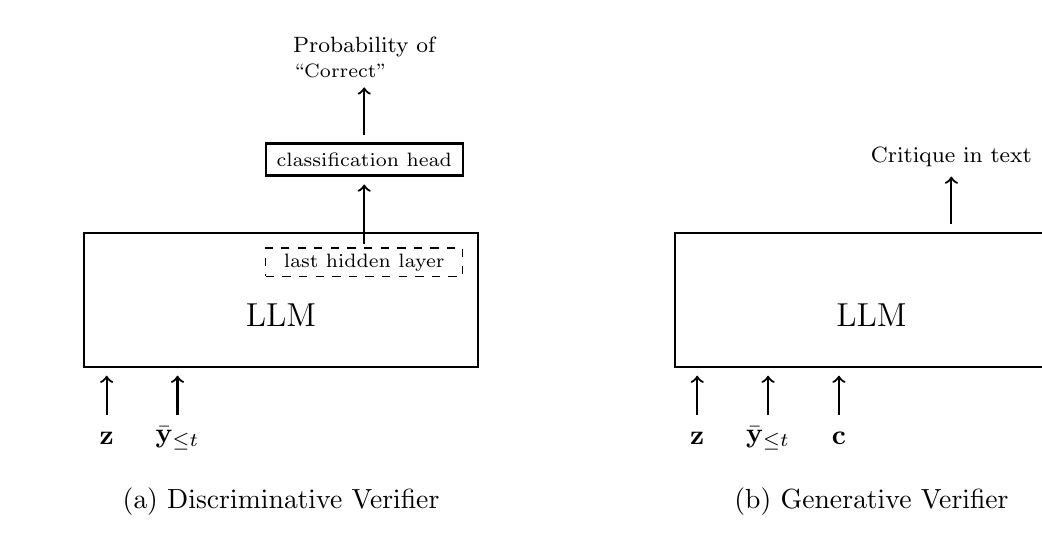
\begin{tikzpicture}
	
\def\ssep{0.3cm}

\tikzstyle{lnode} = [minimum width=5.0cm,minimum height=1.7cm,draw,thick,inner sep=2pt];

%%% scalar verifier
\begin{scope}

\node [lnode,anchor=west] (llm) at (0,0) {};
\node [anchor=south] (llmlabel) at ([yshift=0.4cm]llm.south) {\large{LLM}};

\node [anchor=center] (z) at ([xshift=0.3cm,yshift=-0.9cm]llm.south west) {$\mathbf{z}$};
\node [anchor=center] (steps) at ([xshift=0.9cm]z.center) {$\bar{\mathbf{y}}_{\le t}$};
%\node [anchor=center] (c) at ([xshift=0.9cm]steps.center) {$\mathbf{c}$};

\draw [->,thick] ([yshift=0.3cm]z.center) -- ([yshift=0.8cm]z.center);
\draw [->,thick] ([yshift=0.3cm]steps.center) -- ([yshift=0.8cm]steps.center);
%\draw [->,thick] ([yshift=0.3cm]c.center) -- ([yshift=0.8cm]c.center);

\node [anchor=north east,draw,dashed,minimum width=2.5cm,inner sep=2pt] (hidden) at ([xshift=-0.2cm,yshift=-0.2cm]llm.north east) {\scriptsize{last hidden layer}};

\node [anchor=south,draw,thick,minimum width=2.5cm] (classification) at ([yshift=0.9cm]hidden.north) {\scriptsize{classification head}};
\draw [->,thick] ([yshift=0.05cm]hidden.north) -- ([yshift=-0.1cm]classification.south);

\node [anchor=south,align=left] (prediction) at ([yshift=0.7cm]classification.north) {\footnotesize{Probability of}\\[-0.1cm] \scriptsize{``Correct''}};
\draw [->,thick] ([yshift=0.1cm]classification.north) -- (prediction.south);

\node [anchor=north] (caption) at ([yshift=-1.4cm]llm.south) {(a) Discriminative Verifier};

\end{scope}

%%% generative verifier
\begin{scope}[xshift=7.5cm]

\node [lnode,anchor=west] (llm) at (0,0) {};
\node [anchor=south] (llmlabel) at ([yshift=0.4cm]llm.south) {\large{LLM}};

\node [anchor=center] (z) at ([xshift=0.3cm,yshift=-0.9cm]llm.south west) {$\mathbf{z}$};
\node [anchor=center] (steps) at ([xshift=0.9cm]z.center) {$\bar{\mathbf{y}}_{\le t}$};
\node [anchor=center] (c) at ([xshift=0.9cm]steps.center) {$\mathbf{c}$};

\draw [->,thick] ([yshift=0.3cm]z.center) -- ([yshift=0.8cm]z.center);
\draw [->,thick] ([yshift=0.3cm]steps.center) -- ([yshift=0.8cm]steps.center);
\draw [->,thick] ([yshift=0.3cm]c.center) -- ([yshift=0.8cm]c.center);

\node [anchor=south] (critique) at ([xshift=-1.5cm,yshift=0.7cm]llm.north east) {\footnotesize{Critique in text}};

\draw [->,thick] ([yshift=-0.6cm]critique.south) -- ([yshift=-0.0cm]critique.south);


\node [anchor=north] (caption) at ([yshift=-1.4cm]llm.south) {(b) Generative Verifier};


\end{scope}
	
\end{tikzpicture}

\caption{Comparison between discriminative and generative verification approaches. Subfigure (a) shows a discriminative verifier which attaches a classification head to the last hidden layer of the LLM to output a numerical probability of correctness. Subfigure (b) shows a generative verifier that prompts the LLM with the query $\mathbf{z}$, reasoning history $\bar{\mathbf{y}}_{\le t}$, and an instruction $\mathbf{c}$ to generate a natural language critique instead of a scalar value.}
\label{fig:pre-generative-verfication}
\end{figure}

While natural language critiques are useful for humans, some search algorithms (such as tree search) may require numerical scores to rank different reasoning paths. To extract a continuous score from a generative verifier, a common method is to measure the probability of the model outputting an indicator token (such as ``Correct'' or ``Incorrect'') as the very first word of its critique. Therefore, the numerical verification score can be defined as:
\begin{eqnarray}
v(\mathbf{z}, \bar{\mathbf{y}}_{\le t}, \mathbf{c}) & = & \Pr(y_{\mathrm{anchor}} = \text{``Correct''} | \mathbf{z}, \bar{\mathbf{y}}_{\le t}, \mathbf{c}).
\end{eqnarray}

\noindent Here $y_{\mathrm{anchor}}$ is the indicator token that is typically extracted from the output text using heuristics.

Generative verifiers have several advantages over traditional scalar reward models. First, they provide interpretability for problem solving. Because the verifier explains its reasoning in text, developers can diagnose why a reasoning path is accepted or not. Second, they enable self-correction. Since the text critique often explicitly states how to fix a mistake (like providing the correct expansion $2y + 4$ in our example), the reasoning system can directly integrate this feedback to correct its current state and continue searching, rather than simply discarding the entire path. Third, they require minimal modification of the architecture. As long as current LLMs have strong reasoning capabilities, the exact same model can be used as both the problem solver and the verifier.

\subsubsection{Formal Symbolic Systems as Verifiers}

While neural verifiers are widely used, they share a common weakness: they are still neural networks. This means they can also hallucinate or make logical mistakes. For tasks that require strict precision, such as complex mathematics or software engineering, we can also use formal symbolic systems as verifiers. For example, in code optimization tasks, when a model attempts to optimize intermediate representation code (such as LLVM-IR), a formal equivalency checker (such as Alive2) can automatically verify if the newly generated code maintains the exact same semantics as the original.

Formal systems strictly follow pre-defined mathematical and logical rules, and so their judgments are 100\% reliable. To use a formal system as a verifier, the LLM must generate its reasoning steps as executable code or formal mathematical statements rather than just plain natural language. For example, when solving a math problem, the LLM might write a small Python script to perform a specific intermediate calculation. The system then executes this code using an external tool. The verification process is very straightforward:

\begin{itemize}
\item \vspace{0.5em} If the code runs without errors and produces a valid output, the reasoning step is verified as correct.
\item \vspace{0.3em} If the code throws an error (such as a syntax error or a math violation), the reasoning step is verified as incorrect.
\end{itemize}
\vspace{0.5em}

Formally, let an intermediate step $\bar{\mathbf{y}}_t$ be a generated block of code or formal logic, and let $E$ represent the formal execution environment. The verification score can be defined as:
\begin{eqnarray}
v(\mathbf{x}, \bar{\mathbf{y}}_{<t}, \bar{\mathbf{y}}_t) & = & \begin{cases}
1, & \text{if } E(\bar{\mathbf{y}}_t) \text{  returns the correct result,} \\
0, & \text{otherwise.}
\end{cases}
\end{eqnarray}


This approach has a clear advantage: it eliminates the ``false positives'' caused by verifier hallucinations. Furthermore, when the execution fails, the formal system usually generates an error message. This error message can be fed back into the LLM to help the model understand what went wrong and correct its logic in the next attempt.

However, using formal symbolic systems also comes with limitations. First, it requires the LLM to have strong coding or formalization skills, as translating abstract reasoning into strict code is difficult. Second, while formal systems are perfect for math and coding, they are not suitable for open-ended, real-world tasks (like writing an essay or planning a trip) where reasoning cannot be easily mapped to rigid logical rules.

%----------------------------------------------------------------------------------------
% NEW SECTION
%----------------------------------------------------------------------------------------

\section{Learning to Reason}

Improving the reasoning capabilities of LLMs is challenging, and therefore generally requires a combination of multiple methods. As discussed in the previous section, inference-time scaling aims to activate the ``thinking'' process of existing LLMs during generation. Alternatively, a natural idea is to internalize these reasoning abilities directly into the model parameters during training. In this section, we will focus on this ``learning to reason'' paradigm.

Reasoning data can be incorporated into any training phase. For example, during pre-training, reasoning paths can simply be added as normal text for standard next-token prediction. Also, we can consider reasoning-based training in the post-training phase. For example, during supervised fine-tuning, models can be fine-tuned on high-quality instances of step-by-step problem-solving. This is commonly achieved by training the model on datasets with CoT trajectories. Furthermore, reinforcement learning can be applied to further optimize these reasoning processes. Here we focus on incorporating reasoning-based supervision in LLM alignment. In the following subsections, we will discuss supervised reasoning data, process supervision, reinforcement learning techniques, and strategies for scaling reasoning capabilities.

\subsection{Supervised Reasoning Data}

Formally, in supervised fine-tuning, an LLM is trained on a dataset of input-output pairs $\mathcal{D} = \{(\mathbf{x}, \mathbf{y})\}$. The standard training objective is
\begin{eqnarray}
\hat{\theta} & = & \argmax_{\theta} \sum_{(\mathbf{x}, \mathbf{y}) \in \mathcal{D}} \log \mathrm{Pr}_{\theta} (\mathbf{y}|\mathbf{x}),
\end{eqnarray}

\noindent where $\mathrm{Pr}_{\theta}(\cdot)$ denotes the model parameterized by $\theta$.

If $\mathbf{y}$ is simply the final conclusion, the model learns to predict the answer without explicitly generating the corresponding reasoning path. For reasoning-based training/tuning, we instead redefine $\mathbf{y}$ as a reasoning path. As shown in Eq. (\ref{eq:reasoning-path-notation}), we can represent the output as a reasoning path consisting of a sequence of reasoning steps $\mathbf{y} = \{\bar{\mathbf{y}}_1,...,\bar{\mathbf{y}}_{n_p}\}$. Thus, we can rewrite the above objective as
\begin{eqnarray}
\hat{\theta} & = & \argmax_{\theta} \sum_{(\mathbf{x}, \{\bar{\mathbf{y}}_1,...,\bar{\mathbf{y}}_{n_p}\}) \in \mathcal{D}} \log \mathrm{Pr}_{\theta} (\bar{\mathbf{y}}_1,...,\bar{\mathbf{y}}_{n_p}|\mathbf{x}).
\end{eqnarray}

\noindent In this way, the model is explicitly provided with reasoning details and is trained to generate a complete reasoning path, including the final conclusion.

In practice, to separate the core reasoning process from other parts of the output, reasoning models often use special formatting tokens. A widely adopted approach is to wrap the core reasoning steps inside \texttt{<think>} and \texttt{</think>} tags. When an LLM generates text using this format, the reasoning steps written inside the tags are referred to as a \mindex{CoT trace} (or simply a \mindex{reasoning trace}). We can think of this CoT trace as the scratchpad of the LLM. Just like a student taking a math exam who writes down intermediate calculations on scrap paper before writing the final answer on the official exam sheet, the LLM uses the \texttt{<think>} block to ``show its work''.

For example, a training instance formatted with these tags might look like this:

\vspace{0.5em}
\begin{tcolorbox}[frame empty]
\begingroup
\setlength{\leftskip}{2em}
\setlength{\rightskip}{2em}

What is $15\%$ of $80$?

\vspace{0.3em}

\texttt{<think>}

To calculate this easily, I can break $15\%$ down into $10\%$ and $5\%$.

First, $10\%$ of $80$ is $8$.

Next, $5\%$ is half of $10\%$, which is $4$.

Adding them together: $8 + 4 = 12$.

\texttt{</think>}

The answer is 12.

\endgroup
\end{tcolorbox}
\vspace{0.5em}

Here the query is ``What is $15\%$ of $80$?''. There are five steps in the output, where steps 1-4 represent the CoT trace and step 5 represents the conclusion. Both the \texttt{<think>} and \texttt{</think>} tags are valid tokens, and so the model will learn to generate them to indicate the core reasoning steps. On the user end, we can remove such tags to show a clean output. Note that in practical applications, the output might be very complex and include content not related to reasoning. Therefore, introducing \texttt{<think>} and \texttt{</think>} tags can help the model concentrate on solving the reasoning problem.

Reasoning data can also be represented using various other formats. One straightforward alternative is a natural language step-by-step format. Instead of using special tokens, the data relies on text prefixes, such as ``Step 1:'', ``Step 2:'', or simply ``Thought:'' followed later by ``Answer:''. Furthermore, reasoning data can be structured using role-based message separation. In modern chat templates, instead of mixing the reasoning and the answer in a single message, the reasoning trace is assigned to an internal role (e.g., a ``thought'' or ``system\_scratchpad'' role), while the final conclusion is assigned to the standard ``assistant'' role. This separates the internal thinking of the LLM from the user-facing response at the system level.

\subsection{Process Supervision}

As we discussed in Section \ref{sec:reasoning-verification}, PRMs are powerful tools for verifying reasoning steps during inference. A natural extension is to use it to guide the training of LLMs through process supervision.

In standard outcome supervision (such as supervised fine-tuning), the model is only evaluated on the final outcome of the entire reasoning path $\mathbf{y}$. If the model generates a sequence of five steps and makes a logical error in the third step, an outcome-based training approach might simply penalize the entire sequence. The model is left to guess which exact step caused the failure. This is known as the \textbf{credit assignment problem} \cite{minsky:1961steps,sutton:1984temporal}.

Process supervision solves this by applying training signals at the step level. Instead of a single reward for the whole path, the model receives feedback for every individual step $\bar{\mathbf{y}}_t$. For example, imagine teaching a student to solve a complex algebra equation. If you only look at the final number they write down and say ``Wrong'', the student does not know if they misunderstood the formula, made a simple addition error, or forgot a minus sign. Process supervision is like a teacher pointing specifically to line 3 and saying ``Your logic broke down here''.

Process supervision is typically framed as a reinforcement learning problem. To apply reinforcement learning to process supervision, we generally follow a training loop of three steps:

\begin{itemize}
\item \textbf{Rollout}: The LLM receives an input $\mathbf{x}$ and generates a full reasoning path $\mathbf{y} = \{\bar{\mathbf{y}}_1, \dots, \bar{\mathbf{y}}_{n_p}\}$. The rollout process can be repeated multiple times to generate a set of reasoning paths $\mathcal{Y}$.
\item \textbf{Verification}: A reward model (i.e., a PRM checking intermediate steps) evaluates each path $\mathbf{y}$ and returns a reward score $R(\mathbf{x}, \mathbf{y})$.
\item \textbf{Update}: A reinforcement learning algorithm uses these rewards to update the model parameters $\theta$.
\end{itemize}

A simple training objective can be formalized as maximizing the expected reward
\begin{eqnarray}
J(\theta) & = & \mathbb{E}_{\mathbf{y} \sim \mathrm{Pr}_{\theta}(\cdot|\mathbf{x})} \left[ R(\mathbf{x}, \mathbf{y}) \right]. \label{eq:simple-rl-objective-for-reasoning}
\end{eqnarray}

\noindent We can modify this objective to have more robust training, such as introducing the advantage function into the objective as in PPO.

While this looks like a standard reinforcement learning workflow used in general LLM alignment (as described in Chapter \ChapterLLMTuning), there is a fundamental difference in the nature of the reward. In typical LLM alignment tasks, the reward model usually evaluates the entire generated text and returns a sparse reward at the very end. The reinforcement learning algorithm then struggles with the credit assignment problem, as it has to  guess which tokens or segments actually contributed to that final score.

In contrast, reasoning unfolds step-by-step. Therefore, the verification score, which we will denote as $v_t = v(\mathbf{x}, \bar{\mathbf{y}}_{\le t})$ for simplicity, is inherently a step-level signal. This characteristic makes reasoning tasks well-suited for modern reinforcement learning. Because $v_t$ is generated step by step, it naturally transforms a sparse-reward language generation task into a dense-reward environment.

The main technical question then becomes how to properly transform these natural step-level scores $v_t$ into the formal training signals (such as structured step rewards $r_t$ or advantages $A_t$) required by the algorithms. Depending on the output format of the PRM and the reinforcement learning framework, we consider the following three methods.

\subsubsection{Training with Binary Verification Scores}

In some cases, the PRM acts as a strict rule checker (such as a math calculator or a code compiler). It simply returns a binary score: $v_t \in \{0, 1\}$. A score of $1$ means that the logic at step $t$ is correct given the previous steps, and $0$ means that a logical error occurs at this step.

When dealing with binary scores, the idea is straightforward: a single wrong step invalidates the entire reasoning path. If we want to assign a sequence-level reward $R(\mathbf{x}, \mathbf{y})$ for the whole path, we can simply multiply all the step scores together
\begin{eqnarray}
R(\mathbf{x}, \mathbf{y}) & = & \prod_{t=1}^{n_p} v_t.
\end{eqnarray}

\noindent Hence the model only gets a positive reward if the verification score of every single step is $1$.

Alternatively, if the reinforcement learning algorithm supports step-level rewards (denoted as $r_t$), we can penalize the model exactly where the failure happens. For example, we can give a reward of $1$ as long as the steps remain correct ($v_t = 1$). The moment the model makes a mistake ($v_t = 0$), we assign a negative reward and stop the generation.


\subsubsection{Training with Real-valued Verification Scores}

In most neural PRMs, the verifier outputs a continuous real number $v_t \in \mathbb{R}$. This could be a probability from $0$ to $1$ (indicating the confidence that the reasoning path is correct) or an unnormalized scalar value.

To apply continuous verification scores, the most common technique is \textbf{reward shaping}. Instead of using absolute scores, we define the immediate step reward $r_t$ as the marginal difference between the current step and the previous step:
\begin{eqnarray}
r_t & = & v_t - v_{t-1}.
\end{eqnarray}

This method is very intuitive. Imagine a PRM estimating the probability of getting the final answer right. If Step 1 has a confidence of $0.4$, and Step 2 contains a brilliant deduction that raises the confidence to $0.9$, the reward for Step 2 is $r_2 = 0.9 - 0.4 = +0.5$. The model is rewarded for that specific logical leap. If Step 3 introduces a calculation error and the confidence drops to $0.1$, the reward is $r_3 = 0.1 - 0.9 = -0.8$.

When we sum these shaped rewards across the entire sequence, we have a ``telescoping sum'' that forms our sequence-level reward $R(\mathbf{x}, \mathbf{y})$:
\begin{eqnarray}
R(\mathbf{x}, \mathbf{y}) & = & \sum_{t=1}^{n_p} r_t \nonumber \\
& = & (v_1 - v_0) + (v_2 - v_1) + \dots + (v_{n_p} - v_{n_p-1}) \nonumber \\
& = & v_{n_p} - v_0.
\end{eqnarray}

\noindent Here, $v_0$ is generally assumed to be 0. In this derivation, the intermediate scores cancel out. This means that the overall sequence reward remains consistent with the evaluation of the final step.

To understand how this step-by-step dense reward actually trains the model, we need to connect it to the reinforcement learning objective. As is shown in Eq. (\ref{eq:simple-rl-objective-for-reasoning}), our goal is to maximize the expected total reward over all possible generated paths. To make training efficient and have proper credit assignment, we typically use the principle of causality: an action taken at step $t$ can only affect the rewards received after this step. Therefore, rather than evaluating a step using the entire sequence reward, we evaluate it using the future return $R_t$, which is defined as the sum of rewards from step $t$ to the end of the sequence:
\begin{eqnarray}
R_t & = & \sum_{k=t}^{n_p} r_k \nonumber \\
& = & v_{n_p} - v_{t-1}.
\end{eqnarray}

Finally, we can train the model using the surrogate loss function
\begin{eqnarray}
\mathcal{L}(\theta) & = & - \sum_{t=1}^{n_p} \log \mathrm{Pr}_{\theta}(\bar{\mathbf{y}}_t | \mathbf{x}, \bar{\mathbf{y}}_{<t}) \cdot R_t.
\end{eqnarray}

This loss function provides a step-level feedback mechanism. For any generated reasoning path, the model looks at the future return $R_t$ at each step $t$. If $R_t$ is positive, the loss function pushes the model to increase the probability $\log \mathrm{Pr}_\theta(\cdot)$ of generating this step. If $R_t$ is negative, it serves as a penalty, which pushes the model to avoid generating this step in the future.


\subsubsection{Incorporating Verification into the Advantage Function}

Many reinforcement learning algorithms (such as PPO) optimize the model using the advantage function $A_t$, which measures how much better an action was compared to what was expected. Instead of treating verification scores as raw rewards, we can incorporate them into the advantage calculation.

One method is to introduce step-level verification into the temporal difference error. If the PRM is trained to estimate the expected future reward, we can treat it as the value baseline in standard actor-critic reinforcement learning. We calculate the advantage $A_t$ using the temporal difference error
\begin{eqnarray}
A_t & = & \tilde{r}_{t} + \gamma v_t - v_{t-1},
\end{eqnarray}

\noindent where $\tilde{r}_{t}$ is any external reward from the environment (usually $0$ during intermediate thinking steps) and $\gamma$ is the discount factor.

Another method is to improve the design of the group relative advantage. In \mindex{group relative policy optimization} (\mindex{GRPO}), we dispense with absolute verification scores \cite{shao-etal:2024deepseekmath}. Instead, we compute the advantage by comparing a group of reasoning paths. For an input $\mathbf{x}$, the LLM generates a group of different reasoning paths. A verifier assigns a score $v_t^{(i)}$ to the $t$-th step of the $i$-th path. The advantage $A_t^{(i)}$ is calculated by accumulating the standardized scores from step $t$ to the end of the path, as follows
\begin{eqnarray}
A_t^{(i)} & = & \sum_{k = t}^{n_p^{(i)}} \tilde{v}_k^{(i)},
\end{eqnarray}

\noindent where $n_p^{(i)}$ is the total number of steps in the $i$-th path, and $\tilde{v}_k^{(i)}$ is the standardized score, defined as:
\begin{eqnarray}
\tilde{v}_k^{(i)} & = & \frac{v_k^{(i)} - \mu}{\sigma},
\end{eqnarray}

\noindent where $\mu$ and $\sigma$ are the mean and standard deviation of the scores across all steps of the paths in the group. For example, if a model explores 5 different ways to solve an equation, and path \#3 executes a step that scores significantly higher than the average of all steps in these paths, path \#3 receives a positive advantage. Here, the group average $\mu$ serves as the baseline, which removes the need to train and run a separate value network.


Once the advantage $A_t$ (or $A_t^{(i)}$) is calculated using either of these methods, it can be used as the scaling weight in the loss function. A simplified version of the advantage-based loss function can be written as\footnote{Note that advanced algorithms like PPO and GRPO usually enhance this objective by adding a clipping mechanism (restricting the probability ratio between the new and old policies) to prevent the model parameters from changing too drastically in a single update. However, the core mathematical principle remains the same.}:
\begin{eqnarray}
\mathcal{L}(\theta) & = & - \sum_{t=1}^{n_p} \log \mathrm{Pr}_{\theta}(\bar{\mathbf{y}}_t | \mathbf{x}, \bar{\mathbf{y}}_{<t}) \cdot A_t.
\end{eqnarray}

Note that the benefit of using the advantage $A_t$ over the raw return $R_t$ is variance reduction. By subtracting a baseline, whether it is an estimated value $v_{t-1}$ or a group average $\mu$, the advantage function provides a relative performance measure. It tells the model not just whether a reasoning step is logically sound, but whether it is better than expected. This relative feedback prevents the model from being overwhelmed by queries that are too easy or too hard.

\subsection{On-Policy Distillation for Reasoning}

While process supervision provides step-by-step reward signals to guide reasoning, it still relies on a scalar value to tell the model how well it is doing. To provide an even richer training signal, we can employ \mindex{on-policy distillation} (\mindex{OPD}). This method is generally used in post-training of LLMs, and aligns well with the goal of step-based supervision: making the training signals as dense as possible.

Standard knowledge distillation can be viewed as a kind of \mindex{off-policy distillation}. A smaller ``student'' model learns by mimicking the reasoning paths generated by a stronger ``teacher'' model. The student is trained on a fixed dataset of these pre-recorded paths. However, reasoning is a long and fragile process. If the student makes a small mistake or chooses a slightly different valid approach during actual generation, it enters a state it has never seen in the training data. Because the student does not know how to recover from its mistakes, the reasoning process may collapse. This phenomenon is known as exposure bias or distribution shift.

The core idea of OPD is that the student model learns from its own generated trajectories, rather than from trajectories sampled from the teacher model. Formally, let the teacher model be $\mathrm{Pr}^{t}(\cdot)$ and the student model (parameterized with $\theta$) be $\mathrm{Pr}_{\theta}^{s}(\cdot)$. The typical procedure of OPD consists of two steps:

\begin{itemize}
\item \vspace{0.5em} \textbf{Student Rollout}. Given an input $\mathbf{x}$, the student model uses its current parameters $\theta$ to generate a reasoning path $\mathbf{y} = \{\bar{\mathbf{y}}_1, \dots, \bar{\mathbf{y}}_{n_p}\}$. Because the student generates this path itself, it naturally explores its own reasoning behaviors. This includes making slight deviations, taking alternative approaches, or even making mistakes that a teacher would never make.
\item \vspace{0.3em} \textbf{Teacher Guidance}. We then feed this student-generated path to the teacher model. At each step $t$, instead of providing a scalar reward, the teacher model calculates the probability distribution for the next step $\mathrm{Pr}^{t}(\cdot | \mathbf{x}, \bar{\mathbf{y}}_{<t})$.
\end{itemize}
\vspace{0.5em}

Ideally, the student model is updated to align its step-level probability distribution with the distribution generated by the teacher model. The objective is to minimize the expected KL divergence between the two distributions over the reasoning paths generated by the student model:
\begin{eqnarray}\mathcal{L}_{\mathrm{step}}(\theta) & = & \mathbb{E}_{\mathbf{y} \sim \mathrm{Pr}_{\theta}^{s}(\cdot|\mathbf{x})} \left[ \sum_{t=1}^{n_p} D_{\mathrm{KL}} \left( \mathrm{Pr}_{\theta}^{s}(\cdot | \mathbf{x}, \bar{\mathbf{y}}_{<t}) \,\|\, \mathrm{Pr}^{t}(\cdot | \mathbf{x}, \bar{\mathbf{y}}_{<t}) \right) \right].
\end{eqnarray}

\noindent However, calculating this step-level distribution is computationally intractable in practice. Because a reasoning step $\bar{\mathbf{y}}_t$ typically consists of multiple tokens, the probability distribution over all possible multi-token steps resides in an exponentially large space.

To address this, we fall back to the standard OPD approach, which operates at the token level. By treating the generated reasoning path as a token sequence $\mathbf{y} = \{y_1,\dots, y_n\}$, the objective is reformulated to compute the KL divergence token by token over the vocabulary:
\begin{eqnarray}
\mathcal{L}_{\mathrm{token}}(\theta) & = & \mathbb{E}_{\mathbf{y} \sim \mathrm{Pr}_{\theta}^{s}(\cdot|\mathbf{x})} \left[ \sum_{i=1}^{n} D_{\mathrm{KL}} \left( \mathrm{Pr}_{\theta}^{s}(\cdot | \mathbf{x}, \mathbf{y}_{<i}) \,\|\, \mathrm{Pr}^{t}(\cdot | \mathbf{x}, \mathbf{y}_{<i}) \right) \right].
\end{eqnarray}

\noindent This objective is then approximated using sampling. For a given input $\mathbf{x}$, we simply perform a rollout to generate one (or a small batch of) reasoning paths from the student model, and calculate the token-level KL divergence on these sampled rollouts.

Figure \ref{fig:comparision-of-sft-ps-opd} compares OPD with supervised fine-tuning and process supervision. To further understand the difference among these methods, imagine a student trying to solve a complex geometry problem:

\begin{figure}[!t]
\centering
% !Mode:: "TeX:UTF-8"
% !TEX encoding = UTF-8 Unicode

\begin{tikzpicture}
	
\def\ssep{1.0cm}

\tikzstyle{mnode} = [minimum width=1.8cm,minimum height=0.8cm,draw,thick,inner sep=3pt];
\tikzstyle{wnode} = [minimum width=0.4cm,minimum height=0.4cm,inner sep=2pt];

%%% sft
\begin{scope}

\node [mnode,anchor=west] (student) at (0,0) {\small{Student}};
\node [mnode,anchor=south,align=left] (teacher) at ([yshift=1.5cm]student.north) {\small{Human/}\\[-3pt]\small{Teacher}};

\node [anchor=west,wnode] (w1) at ([xshift=3cm]teacher.east) {\small{This}};
\node [anchor=center,wnode] (w2) at ([xshift=\ssep]w1.center) {\small{cat}};
\node [anchor=center,wnode] (w3) at ([xshift=\ssep]w2.center) {\small{is}};
\node [anchor=center,wnode] (w4) at ([xshift=\ssep]w3.center) {\small{cute}};
\node [anchor=center,wnode] (w5) at ([xshift=\ssep]w4.center) {\small{.}};

\begin{pgfonlayer}{background}
\node [draw, rounded corners=1mm]  [fit = (w1) (w5)] (ty) {};
\end{pgfonlayer}

\draw [->] ([xshift=1pt]teacher.east) -- ([xshift=-1pt]ty.west) node [pos=0.5,above] {\footnotesize{Annotate/Generate}};
\node [anchor=south] (tylabel) at (ty.north) {\footnotesize{Target Output ($\mathbf{y}^*$)}};

\draw [<->,blue,thick,dashed] ([xshift=-1cm,yshift=-1pt]ty.south) .. controls +(south:1.7cm) and +(east:2cm) .. ([xshift=1pt]student.east) node [pos=0.5,right,align=left,xshift=0.8cm,yshift=-0.1cm] {\footnotesize{Teacher forcing}\\[-1pt] \footnotesize{$\max\limits_{\theta} \Pr_{\theta}^s(\mathbf{y}^*|\mathbf{x})$}};

\node [anchor=north] (caption) at ([xshift=3cm,yshift=-0.5cm]student.south east) {\small{(a) Supervised Fine-tuning}};

\end{scope}

%%% process supervision
\begin{scope}[yshift=-5.2cm]

\node [mnode,anchor=west] (student) at (0,0) {\small{Student}};

\node [anchor=west,wnode] (w1) at ([xshift=3cm]student.east) {\small{The}};
\node [anchor=center,wnode] (w2) at ([xshift=\ssep]w1.center) {\small{cat}};
\node [anchor=center,wnode] (w3) at ([xshift=\ssep]w2.center) {\small{is}};
\node [anchor=center,wnode,fill=gray!30] (w4) at ([xshift=\ssep,yshift=-0.05cm]w3.center) {\small{lovely}};
\node [anchor=center,wnode] (w5) at ([xshift=\ssep,yshift=0.05cm]w4.center) {\small{.}};

\begin{pgfonlayer}{background}
\node [draw, rounded corners=1mm]  [fit = (w1) (w5)] (sy) {};
\end{pgfonlayer}

\draw [->] ([xshift=1pt]student.east) -- ([xshift=-1pt]sy.west) node [pos=0.5,above] {\footnotesize{Generate}};
\node [anchor=north] (sylabel) at (sy.south) {\footnotesize{Output of the student model ($\mathbf{y}$)}};

\node [mnode,anchor=south] (verifier) at ([yshift=2.0cm]w4.north) {\small{Verifier}};

\draw [->] ([yshift=-1pt]verifier.south) -- ([yshift=0pt]w4.north) node (verificationlabel) [pos=0.4,left,align=right] {\footnotesize{Generate the verification}\\[-2pt]\footnotesize{score $v_t$ and compute }\\[-2pt]\footnotesize{the advantage $A_t$}};

\draw [<->,blue,thick,dashed] ([yshift=1pt]student.north) .. controls +(north:1cm) and +(west:2cm) .. ([yshift=0.3cm]verificationlabel.west) node [pos=0.3,above,yshift=0.3cm,align=right] {\footnotesize{Training with RL}\\[-1pt]\footnotesize{$\max\limits_{\theta} \sum_{t=1}^{n_p} \log \mathrm{Pr}_{\theta}(\bar{\mathbf{y}}_t | \mathbf{x}, \bar{\mathbf{y}}_{<t}) \cdot A_t$}};

\node [anchor=north] (caption) at ([xshift=3cm,yshift=-0.5cm]student.south east) {\small{(b) Process Supervision}};

\end{scope}

%%% odp
\begin{scope}[yshift=-10.4cm]

\node [mnode,anchor=west] (student) at (0,0) {\small{Student}};

\node [anchor=west,wnode] (w1) at ([xshift=3cm]student.east) {\small{The}};
\node [anchor=center,wnode] (w2) at ([xshift=\ssep]w1.center) {\small{cat}};
\node [anchor=center,wnode] (w3) at ([xshift=\ssep]w2.center) {\small{is}};
\node [anchor=center,wnode,fill=gray!30] (w4) at ([xshift=\ssep,yshift=-0.05cm]w3.center) {\small{lovely}};
\node [anchor=center,wnode] (w5) at ([xshift=\ssep,yshift=0.05cm]w4.center) {\small{.}};

\begin{pgfonlayer}{background}
\node [draw, rounded corners=1mm]  [fit = (w1) (w5)] (sy) {};
\end{pgfonlayer}

\draw [->] ([xshift=1pt]student.east) -- ([xshift=-1pt]sy.west) node [pos=0.5,above] {\footnotesize{Generate}};
\node [anchor=north] (sylabel) at (sy.south) {\footnotesize{Output of the student model ($\mathbf{y}$)}};

\node [mnode,anchor=south] (teacher) at ([yshift=2.0cm]w4.north) {\small{Teacher}};

\node [anchor=south,minimum width=0.2cm,minimum height=0.4cm,fill=orange!30] (sh3) at ([yshift=0.5cm]w4.north) {};
\node [anchor=south east,minimum width=0.2cm,minimum height=0.3cm,fill=orange!30] (sh2) at ([xshift=-1pt]sh3.south west) {};
\node [anchor=south east,minimum width=0.2cm,minimum height=0.2cm,fill=orange!30] (sh1) at ([xshift=-1pt]sh2.south west) {};
\node [anchor=south west,minimum width=0.2cm,minimum height=0.2cm,fill=orange!30] (sh4) at ([xshift=1pt]sh3.south east) {};
\node [anchor=south west,minimum width=0.2cm,minimum height=0.3cm,fill=orange!30] (sh5) at ([xshift=1pt]sh4.south east) {};

\node [anchor=south,minimum width=0.2cm,minimum height=0.3cm,fill=purple!30] (th3) at ([yshift=1.2cm]w4.north) {};
\node [anchor=south east,minimum width=0.2cm,minimum height=0.2cm,fill=purple!30] (th2) at ([xshift=-1pt]th3.south west) {};
\node [anchor=south east,minimum width=0.2cm,minimum height=0.4cm,fill=purple!30] (th1) at ([xshift=-1pt]th2.south west) {};
\node [anchor=south west,minimum width=0.2cm,minimum height=0.3cm,fill=purple!30] (th4) at ([xshift=1pt]th3.south east) {};
\node [anchor=south west,minimum width=0.2cm,minimum height=0.2cm,fill=purple!30] (th5) at ([xshift=1pt]th4.south east) {};

\draw [->] ([yshift=1pt]w4.north) -- ([yshift=-1pt]sh3.south);
\draw [->] ([yshift=-1pt]teacher.south) -- ([yshift=-0.3cm]teacher.south);

\node [anchor=south west,align=left,inner sep=2pt] (tdislabel) at ([yshift=-0.1cm,xshift=0.1cm]th5.south east) {\tiny{Teacher's predicted}\\[-6pt]\tiny{Distribution $\mathrm{Pr}^{t}(\cdot | \mathbf{x}, \mathbf{y}_{<i})$}};
\node [anchor=south west,align=left,inner sep=2pt] (sdislabel) at ([yshift=-0.1cm,xshift=0.1cm]sh5.south east) {\tiny{Student's predicted}\\[-6pt]\tiny{Distribution $\mathrm{Pr}^{s}(\cdot | \mathbf{x}, \mathbf{y}_{<i})$}};

\draw [<->,blue,thick,dashed] ([yshift=1pt]student.north) .. controls +(north:1.2cm) and +(west:3cm) .. ([xshift=-1pt]th1.west) node [pos=0.2,above,yshift=0.4cm,xshift=1.2cm,align=right] {\footnotesize{Minimizing the KL divergence}\\[-1pt]\footnotesize{$\min\limits_{\theta} \sum_{i=1}^{n} D_{\mathrm{KL}} \left( \mathrm{Pr}_{\theta}^{s}(\cdot | \mathbf{x}, \mathbf{y}_{<i}) \parallel \mathrm{Pr}^{t}(\cdot | \mathbf{x}, \mathbf{y}_{<i}) \right)$}};


\node [anchor=north] (caption) at ([xshift=3cm,yshift=-0.5cm]student.south east) {\small{(c) On-policy Distillation}};

\end{scope}
	
	
\end{tikzpicture}

\caption{Comparison of supervised fine-tuning, process supervision, and on-policy distillation methods. In supervised fine-tuning (a), the student model is trained off-policy to maximize the likelihood of golden target outputs provided by a human or a teacher model. In process supervision (b), the student model generates its own reasoning path, and a verifier evaluates these self-generated steps to compute advantages. In on-policy distillation (c), the student also generates its own path, but instead of scalar rewards, a teacher model provides a dense, token-level probability distribution at each step. The student is updated by minimizing the KL divergence between its own predicted distribution and the teacher's distribution.}
\label{fig:comparision-of-sft-ps-opd}
\end{figure}

\begin{itemize}
\item \vspace{0.5em} \textbf{Supervised Fine-tuning}. This is like giving the student a textbook filled with the correct solutions written by the teacher to memorize. If the student decides to draw an auxiliary line differently than the textbook did, the textbook offers no help on how to proceed from that new starting point.
\item \vspace{0.5em} \textbf{Process Supervision} (RL with PRMs). This is like having a strict grader who checks the student's work step-by-step and says, ``+1 point for step 1'', and ``-1 point for step 2''. It tells the student where they went wrong, but not how to fix it or what the correct next step should be.
\item \textbf{On-Policy Distillation}. This is like having an expert tutor sitting right next to the student. When the student draws that unusual auxiliary line (a state not in the standard textbook), the tutor looks at the student's current state and says, ``Okay, since you drew the line here, your next best step is to calculate this specific angle.''
\end{itemize}

Because the supervision of OPD comes in the form of a full probability distribution over the vocabulary, the student receives a very dense and rich learning signal. It learns not only what the single best next step is, but also the probabilities of other valid alternatives. This rich feedback is well suited for reasoning because it teaches the student model how to recover from deviations and maintain logical consistency across the entire output sequence, rather than just treating a rationale as an isolated component. However, applying on-policy distillation comes with a high computational cost. The process requires running a large teacher model alongside the student during training to calculate probability distributions in real time. This is more expensive than standard off-policy distillation, where the outputs of the teacher model are only generated once and stored in a static dataset.

\subsection{Scaling Training for Reasoning}

Scaling is a core strategy in the era of LLMs. When dealing with complex reasoning tasks, scaling the training process is a natural idea. Here, we briefly discuss several key aspects of scaling training for reasoning LLMs: large-scale reinforcement learning, synthetic data generation, and long-context scaling.

\subsubsection{Large-scale Reinforcement Learning}

Reinforcement learning has become a primary approach to improving the ``System 2'' reasoning abilities of LLMs. For example, the success of many powerful reasoning models comes from scaling up reinforcement learning rather than using supervised fine-tuning only. An interesting phenomenon observed during large-scale reinforcement learning-based training is the emergence of the ``aha moment''~\cite{deepseek:2025r1}. Without explicit human annotation, LLMs learn to pause, recognize when they have made a mistake, or even backtrack to try a different approach. These abilities are difficult to elicit when relying solely on limited labeled data and standard supervised training. As training compute scales, the model can allocate longer CoT traces to harder problems, and thus discover how to think deeply on its own~\cite{snell-etal:2024scaling}.

Recent large-scale empirical studies have demonstrated that the relationship between reinforcement learning compute and reasoning performance can be modeled by an S-shaped curve \cite{khatri-etal:2025art,tan-etal:2026scaling}. A key finding from this scaling law is that different training choices impact the curve differently. For instance, increasing the base capabilities of the LLM (e.g., using larger architectures or MoEs) and expanding the context window length can increase the performance limit. Conversely, algorithmic improvements, such as changing the loss function or adjusting advantage normalization, mainly make better use of the available compute budget but do not significantly improve the final performance.

Scaling reinforcement learning is difficult. First, the computational cost is very high. For every training sample, the system generally performs a rollout (running the model for inference) and then calls an extra reward model or another LLM to evaluate the generated output. When the number of training samples increases, this cost becomes significantly higher than that of standard supervised fine-tuning. This computational burden also makes running experiments and trial-and-error much more difficult. Furthermore, reinforcement learning methods are generally complex and require very careful tuning to achieve good results. For example, they are sensitive to hyperparameter settings and training data. As a result, reinforcement learning methods are relatively fragile. When training on a massive scale, ensuring that the system runs stably (for instance, making sure the training loss decreases steadily) is not just a machine learning problem, but also an engineering challenge.

\subsubsection{More Synthetic Data for Reasoning}

Because high-quality human annotations for complex multi-step reasoning are scarce, scaling training data often relies on synthetic data generation. Instead of manually writing step-by-step proofs, researchers use strong LLMs to generate diverse reasoning trajectories, which are then filtered and curated to train new models~\cite{zelikman-etal:2022star,mukherjee-etal:2023orca}.

To generate synthetic data for reasoning, a common approach is to sample multiple reasoning paths from teacher models for a given seed question~\cite{wang-etal:2023self}. We can then apply verifiers or execution environments to evaluate these paths, and retain only those that arrive at the correct final answer through sound logical steps. Furthermore, models can be used to generate variations of existing problems (e.g., changing numerical values or structural constraints in math and coding tasks) to expand the distribution of training data.

\subsubsection{Scaling Context Length}

As reasoning models tackle increasingly complex problems, the length of reasoning paths has become a primary bottleneck. The demand for large context windows in reasoning arises from several sources. First, to elicit deep System 2 thinking, the input prompt itself often requires extensive context. This includes detailed logical constraints, complex environment rules, or multiple long few-shot CoT examples. Second, the generated reasoning process for a complex task can easily span thousands or even tens of thousands of tokens before arriving at the final conclusion. Third, recent advances in LLM agents have also increased the demand for reasoning. Agentic reasoning often extends over many rounds of interaction, creating an even greater need for long context windows.

This demand has directly driven the LLM industry to develop models that support massive context windows. For instance, many LLMs now support context lengths of up to 128K tokens, and more advanced models, such as Anthropic's Claude 3.5~\cite{anthropic:2024claude35} and Google's Gemini 1.5~\cite{gemini:2024gemini}, support hundreds of thousands of tokens, or even one million tokens. The interested reader may refer to Chapter \ChapterLLM\ for a more detailed discussion on long-context LLMs.

However, handling long contexts for reasoning leads to new challenges that go beyond general context compression. In tasks like summarizing a long novel or extracting key points from documents, an LLM can afford to compress information and lose minor details. In contrast, reasoning requires strict, high-precision logical continuity. Every intermediate step is a critical link in a heavily interdependent chain. If the model ``forgets'' a specific assumption defined in the prompt, or loses track of a variable calculated in step 2 while executing step 50, the entire derivation collapses. Therefore, scaling context for reasoning is not just about expanding the KV cache to store more tokens. It requires the model to achieve reliable retrieval across long distances and to maintain strict logical consistency.

%----------------------------------------------------------------------------------------
% NEW SECTION
%----------------------------------------------------------------------------------------

\section{Evaluating Reasoning LLMs}

In this section, we discuss how to evaluate reasoning LLMs. This task is similar to evaluating standard LLMs \cite{chang-etal:2024survey}. However, reasoning problems are so complex that we often need more detailed evaluation and other special considerations.

\subsection{Outcome-based vs. Process-based Evaluation}

When evaluating how well an LLM reasons, the easiest and most common method is \textbf{outcome-based evaluation}. In this approach, we only look at the final answer produced by the model. If the final answer matches the ground truth, the model is considered correct. This method is widely used in popular reasoning benchmarks, such as GSM8K \cite{cobbe-etal:2021training} and MATH \cite{hendrycks-etal:2measuring}. However, outcome-based evaluation has the ``right answer for the wrong reason'' problem, also known as a false positive. A model might generate flawed logical steps but accidentally arrive at the correct final number. If we only check the final outcome, we might incorrectly conclude that the model possesses strong reasoning capabilities when it just got lucky.

For more detailed evaluation, we can use \textbf{process-based evaluation}. Instead of just checking the final answer, we can examine the entire reasoning path step by step \cite{wang-etal:2024math,xia-etal:2025evaluating}. A model is only considered correct if both its intermediate logic and its final conclusion are sound. This is an ideal method but is very difficult to implement in practice. The main challenge is that step-level ``gold data'' is scarce and expensive to create. Furthermore, for any complex problem, there is an exponentially large number of valid reasoning paths. It is infeasible to manually list all correct intermediate steps for every path a model might take.

To make process-based evaluation more practical, we can narrow the scope to evaluate local reasoning decisions. One approach is to reduce the problem to a simple next-step evaluation task: given a correct sequence of previous steps, we check whether the reasoning model can correctly choose or generate the next logical step. To do this, it is straightforward to use PRMs to evaluate the quality of each step generated by the LLM. This method is also related to reward model evaluation \cite{lambert-etal:2025rewardbench}. Instead of examining the output of the reasoning model, we assess the quality of the PRMs. Furthermore, we can consider the fundamental capabilities of reasoning models, such as their ability to identify errors in a given reasoning path. This can also be viewed as a test of their meta-reasoning abilities: we ask the model not just to reason, but to evaluate the reasoning process itself \cite{zeng-etal:2024mr}.

In practice, process-based evaluation is not based on a single standard. We can judge the quality of a reasoning step from different angles, such as logical consistency, coherence, and objectivity \cite{lee-and-hockenmaier:2025evaluating}. However, while process-based evaluation is much more detailed, it comes with a much higher annotation cost, and is often not robust enough. Therefore, most real-world research still relies on the simpler outcome-based evaluation.

\subsection{Evaluation Metrics}

Here we list some metrics used for evaluating reasoning LLMs.

\begin{itemize}
\item \vspace{0.5em} \textbf{Exact Match and Accuracy:} This is the simplest and most widely used metric for tasks with definitive final answers, such as math word problems. Suppose we have a dataset $\mathcal{D}$ consisting of $N$ problems. For the $i$-th problem, we extract the final answer $\hat{a}_i$ from the generated reasoning path and compare it to the ground truth $a_i^*$. The accuracy is defined as:
\begin{eqnarray}
\text{Accuracy} & = & \frac{1}{N} \sum_{i=1}^N \mathbbm{1}(\hat{a}_i = a^*_i).
\end{eqnarray}

\noindent In practice, the exact match method (checking if the strings are perfectly identical) can be too strict, for example, we reject ``$0.5$'' when the ground truth is ``$1/2$''. Therefore, researchers usually apply rule-based scripts to normalize the answers into a canonical format before comparison.

\item \vspace{0.3em} \textbf{Pass@$k$:} Because LLMs are probabilistic, a single decoding attempt might fail in reasoning due to a minor error. Pass@$k$ measures the probability that the model can find at least one correct answer if it is allowed to generate $k$ independent reasoning paths \cite{chen-etal:2021evaluating}. This metric is especially popular in code generation and complex math tasks. For the $i$-th problem in $\mathcal{D}$, if we sample $N_s \ge k$ paths and $C_i$ of them contain the correct answer, the Pass@$k$ score is defined as:
\begin{eqnarray}
\text{Pass}@k & = &  \frac{1}{N} \sum_{i=1}^N \left( 1 - \frac{\binom{N_s-C_i}{k}}{\binom{N_s}{k}} \right).
\end{eqnarray}

\noindent To generate multiple different reasoning paths, we can use the sampling methods described in Section \ref{sec:sampling-reasoning-paths}.

\item \vspace{0.3em} \textbf{Cons@$k$ (Consensus@$k$):} Unlike Pass@$k$, which requires an oracle to verify whether each of the $k$ sampled answers is correct, Cons@$k$ constructs a consensus answer without identifying the correctness of individual samples. Specifically, we generate $k$ reasoning paths, extract their final answers, and select the most frequent answer through majority voting \cite{wang-etal:2023self}. The consensus answer $\hat{a}_i^{\text{maj}}$ for the $i$-th problem is defined as:
\begin{eqnarray}
\hat{a}_i^{\text{maj}} & = & \argmax_{a_i} \sum_{j=1}^k \mathbbm{1}(\hat{a}_i^j = a_i),
\end{eqnarray}

\noindent where $\hat{a}_i^j$ is the final answer extracted from the $j$-th reasoning path. The final accuracy is then obtained by comparing $\hat{a}_{\text{maj}}$ with the ground truth:
\begin{eqnarray}
\text{Cons}@k & = & \frac{1}{N} \sum_{i=1}^N \mathbbm{1}(\hat{a}_i^{\text{maj}} = a^*_i).
\end{eqnarray}

Cons@$k$ provides a practical evaluation approach for real-world reasoning systems, as it measures whether a model can consistently arrive at the correct answer. Compared with Pass@$k$, which evaluates whether at least one sampled response is correct, Cons@$k$ emphasizes the reliability of reasoning by favoring answers that are consistently supported across multiple sampled reasoning paths.

\item \vspace{0.3em} \textbf{LLM-as-a-Judge:} For open-ended reasoning tasks, such as agentic planning or complex open-domain questions, rule-based exact matching often fails. In such cases, we can employ LLMs as automated judges. For instance, a judge LLM can be prompted to evaluate the generated intermediate steps and score them based on predefined criteria. Alternatively, LLMs can be used to compare two reasoning models. The judge is presented with the outputs from both models for the same query and decides which reasoning path is superior, or if the result is a tie. The win rate then reflects the percentage of times a specific model is preferred.
\end{itemize}
\vspace{0.5em}

\subsection{Open Issues}

One issue is data contamination. As language models are trained on increasingly massive datasets collected from the internet, it becomes very difficult to keep test data out of the training process. If a model has already seen the questions from a reasoning benchmark (like MATH or GSM8K) during its pre-training phase, it might simply be reciting a memorized solution instead of actually reasoning on the fly. This makes it hard to determine whether high benchmark scores reflect true problem-solving abilities or just good memory. To address this, the community is encouraged to explore new benchmarks, where problems are updated continuously, as well as private hold-out sets that are never released to the public.

Another issue is robustness. Current reasoning models are sometimes fragile. A model might solve a complex math problem perfectly, but fail completely if the exact same question is rephrased slightly or if irrelevant details are added to the prompt. This sensitivity suggests that models sometimes rely on superficial text patterns rather than truly understanding the underlying logic. For more robust reasoning, we need LLMs to easily adapt to new or even more challenging tasks.

Moreover, LLMs may generate hallucinated or unfaithful reasoning paths. For example, they might invent fake mathematical rules to reach a conclusion. In some cases, the generated text might look like a perfect logical deduction, but the model actually arrived at the answer via a hidden mechanism (such as a lucky guess or a memorized shortcut). This unfaithfulness highlights a gap between the text the model outputs and its actual internal representations. In reinforcement learning setups, this is often related to the reward hacking problem. If models are only rewarded for the final answer, they often learn to cheat the reward system with flawed logic. Therefore, it is valuable to introduce step-by-step supervision in RL, such as process supervision, to check if each intermediate step is truly correct.

The fourth issue is benchmark saturation. The rapid progress of reasoning LLMs means that standard evaluation benchmarks are quickly becoming outdated. Models are now achieving near-perfect scores on tests that were considered extremely difficult just a year or two ago. This benchmark saturation makes it difficult to compare new models or measure real progress in the field. Therefore, researchers need to develop harder tests that evaluate true logical derivation on novel problems. Note that human-level reasoning is often open-ended and interactive. An alternative approach to testing reasoning models might be to use them in autonomous agents, which can explore, use external tools, and recover from their own errors.

%----------------------------------------------------------------------------------------
% NEW SECTION
%----------------------------------------------------------------------------------------

\section{Remarks}

We now discuss some interesting issues related to reasoning LLMs.

\subsection{External Reasoning vs. Internal Reasoning}

In previous discussions, we assumed that the reasoning process can be well captured by a text-based reasoning path (e.g., CoT). This raises a fundamental question: Does the generated CoT text actually reflect how the model reasons? This inquiry leads us to examine the distinction between externalized reasoning and the true internal ``thinking'' processes.

When we prompt an LLM to think step by step, we are forcing it to externalize its computation into discrete tokens. However, we cannot simply view this text sequence as the actual reasoning process. On one hand, an LLM might generate a detailed and logically sound CoT, but the actual decision-making might have already occurred implicitly within the hidden representations of the very first few tokens. On the other hand, a model might produce a flawed or nonsensical CoT, yet still output the correct final answer, suggesting that its internal representations are tracking the task differently from what the generated text implies.

Researchers have demonstrated that CoT explanations can be deceptive \cite{turpin-etal:2023language,chen-etal:2025reasoning}. For example, LLMs may have bias towards generating a logical CoT to reach an incorrect answer, though the correct answer has been mentioned in the prompt. To uncover how LLMs actually think, researchers are turning to neuron activation analysis and mechanistic interpretability. The goal is to understand what happens inside the hidden layers of an LLM during the generation process. For example, in \citet{frasertaliente-etal:2026natural}'s work, natural language auto-encoders are used to convert the activations into natural language text. A natural language auto-encoder consists of an activation verbalizer and an activation reconstructor, which are used to directly map internal residual stream activations into human-readable text and back. In this way, we can decode these activations to read the thoughts of LLMs.

Another line of research focuses on reasoning without text, called \mindex{latent reasoning} or \mindex{implicit reasoning}. In standard reasoning, as we defined earlier, a reasoning path consists of a sequence of text steps. In latent reasoning, this process happens internally before the model speaks. This is achieved either by replacing discrete tokens with continuous vectors or by generating actual text words in the background that are kept hidden from the user. Here we present some of these methods.

\begin{itemize}
\item \vspace{0.5cm} One of the simplest ideas is the use of ``pause tokens''. As is standard in autoregressive generation, a language model gets one step of internal calculation for every word it outputs. Interestingly, it is discovered that if we feed the model dummy tokens (called pause tokens), the model gets extra computational time to process information in its hidden layers before it has to output the final answer \cite{goyal-etal:2024think}. This shows that LLMs could perform silent computations or latent thinking without generating real words.
\item \vspace{0.3cm} Another approach uses knowledge distillation to compress explicit reasoning into hidden states. For instance, the implicit chain of thought method trains a student model to directly mimic the hidden internal states of a larger teacher model that is thinking out loud \cite{deng-etal:2023implicit}. As a result, the student model learns to skip generating the text. Alternatively, the LLM can also learn from itself using self-distillation techniques \cite{shen-etal:2025codi}. We can force the latent thinking process to match the final hidden states of the text-based reasoning. In both methods, latent thinking is embodied as a continuous mathematical space: instead of generating a step-by-step sequence of readable text, the model computes the reasoning steps using hidden vector-based representations.
\item \vspace{0.3cm} An alternative method to reason in continuous latent spaces is to use the \mindex{chain of continuous thought} (\mindex{COCONUT}) paradigm \cite{hao-etal:2025training}. In standard text generation, the output of the final layer is converted into a discrete token, which is then fed back into the first layer for the next step. This process forces the model to compress its internal computation into a single token. COCONUT bypasses this step during the reasoning phase. It takes the output vector from the last layer and feeds it directly back into the input layer as a \mindex{continuous thought}. By repeating this process, the model builds a chain of continuous vectors before it starts generating the final text answer. Because continuous vectors can hold more information than discrete tokens, the model can explore multiple reasoning paths at the same time without committing to a specific token choice early on. This approach demonstrates that LLMs do not have to rely on human language to solve complex problems. By keeping the reasoning process in a continuous space, they can compute answers more efficiently.
\item \vspace{0.3cm} Instead of performing reasoning in a continuous space, we can also use normal text tokens to represent internal thoughts. For example, in the Quiet-STaR method \cite{zelikman-etal:2024quietstar}, the model is trained to think quietly, right in the middle of reading or writing normal text. The idea is simple: before the model predicts the next token, it generates a short sequence of hidden ``thought'' tokens. You can think of this as an inner monologue or a quick mental scratchpad that the user never sees. After generating these hidden thoughts, the LLM uses them to help guess the actual next word. If these thoughts help the LLM predict the correct word, the LLM is rewarded and learns that this way of thinking is useful. If the thoughts are useless or confusing, the LLM learns to discard them.
\end{itemize}
\vspace{0.5cm}

\subsection{Memorization vs. Reasoning}

When discussing LLMs, a question often arises: Is the model truly ``thinking'', or does it simply have a big memory and is reciting a similar answer it saw in its training data? This leads to the discussion on comparing reasoning and memorization in LLMs.

Simply put, the difference between the two can be summarized as follows:

\begin{itemize}
\item \vspace{0.5cm} Memorization is looking backward. The model adjusts its parameters to learn patterns from the training data. When faced with a similar input, the model simply replays the learned patterns.
\item \vspace{0.3cm} Reasoning is moving forward. Instead of searching for a ready-made answer, the model applies general rules and logic to build a chain of thought step by step. The core of reasoning is generalization, even when facing a completely new problem that never appeared in the training set, the model can solve it using logical tools.
\end{itemize}
\vspace{0.5cm}

In early deep learning research, this boundary was not always clear. For example, \citet{zhang-etal:2021understand} point out that deep neural networks have massive memorization capacity, easily memorizing noisy data with completely random labels. For LLMs, given their huge model sizes, they can not only memorize Wikipedia but also details hidden inside code repositories.

This memorization ability often disguises itself as reasoning. For example, if we prompt an LLM with a classic algorithm problem but tweak the numbers slightly, the LLM might rely on its memory inertia and output the original answer anyway, thus making a basic mistake. This is often referred to as the ``stochastic parrots'' phenomenon~\cite{bender-etal:2021dangers}, which means that the LLM is blindly mimicking and stitching together memorized text without truly understanding the underlying logic.

To better see the difference between memorization and reasoning, we can look at two different dimensions.

\subsubsection{Grokking and Generalization}

When exploring how models transition from memorization to true understanding, researchers has made an interesting discovery called ``grokking''~\cite{power-etal:2022grokking}. They train a small Transformer model to learn binary operations in abstract algebra (such as modular addition). They notice a very interesting phenomenon: early in training, the model quickly reached 100\% accuracy on the training set, but its accuracy on the test set was almost zero. At this stage, the model is clearly just memorizing equations by rote. However, if they do not stop training and let the model continue looping over the data long past the point of overfitting, something surprising happens. Suddenly, the test accuracy spikes to 100\% in a very short time. The model seems to experience an ``aha moment''.


Further studies show that before this ``aha moment'', the model parameters are messily memorizing specific equations (like $2 + 3 = 5$)~\cite{nanda-etal:2023progress}. But when grokking occurs, the network internally develops a general mathematical representation using trigonometric functions and Fourier transforms. It has found a universal algorithm that can explain all the data.

This experiment tells us that reasoning does not appear out of nowhere. It often emerges as a high-level generalization state when memorization hits a bottleneck, or after extensive training, where the network organizes its parameters to find the most universal explanation.

\subsubsection{The Cost Trade-off}

From the perspective of information theory and computational efficiency, LLMs naturally balance memorization and reasoning based on cost. On one hand, memorization requires more parameter capacity. To memorize every fact in the world, the model size would need to grow infinitely. On the other hand, reasoning requires more computational steps at inference time. As long as a model memorizes the general rules of addition and multiplication, it can solve many math problems by taking such computational steps during generation.

Therefore, LLMs usually take the path of least resistance. For common facts, retrieving the answer directly from parameters (or memory) is the fastest way. But for rare, multi-step tasks, using System 2 thinking is a more suitable way.

This also explains why techniques like RAG have become popular. The essence of RAG is to offload the burden of memory to an external database, and thus we can free up the parameter space for reasoning. By separating knowledge retrieval from logical deduction, the LLM no longer needs to memorize ever-changing external facts. Instead, it knows how to look things up and process them.

\subsection{Can LLMs Truly Reason?}

The question of whether LLMs can truly reason is one of the most debated topics in AI today. When we see an LLM perfectly solve a math problem or write a complex schedule, it is very tempting to believe that it understands the world just as a human does. However, to answer this question, we must look at how these models actually work.

Essentially, LLMs work by predicting the next word. Because these models have processed massive amounts of text, they have completely mastered the rules, grammar, and structure of human language. In cognitive science, this is known as \mindex{formal linguistic competence} \cite{chomsky:1965aspects,mahowald-etal:2024dissociating}. They know exactly how words should be logically ordered. However, they struggle with functional linguistic competence, which is the ability to use language to understand and navigate the real world \cite{kambhampati-etal:2024llms}. Unlike humans, who learn by physically interacting with their environment, LLMs only know the underlying patterns of text. Because they are not grounded in the real world, they lack a true understanding of physical space and strict cause-and-effect \cite{mahowald-etal:2024dissociating}.

This limitation becomes obvious when we test LLMs on planning tasks \cite{valmeekam-etal:2023planbench}. For example, for classical planning problems, such as moving colored blocks on a table into a specific stack, the LLM can often solve the problem if it uses common words they had seen in their training data. But if the names of the blocks and the actions are replaced with nonsense words, the performance dropped drastically \cite{kambhampati-etal:2024can}. A true reasoning system would not care about the names, because the underlying mathematical logic is exactly the same. The LLM fails because its familiar text pattern is broken.

Furthermore, techniques like CoT prompting force the model to output a step-by-step process. This shows some behavior of slow and deliberate human thought. But in reality, the LLM is still just moving strictly forward, and predicts what a logical explanation usually looks like. If the LLM makes a mistake or holds a biased assumption, it will often confidently generate a flawed explanation simply to justify its wrong answer \cite{chen-etal:2025reasoning}.

Ultimately, to answer whether LLMs can ``truly'' reason, we first need to define what true reasoning actually means. If we expect LLMs to think exactly like humans, it is clear from the discussion above that there are some differences. However, if we view reasoning purely as a functional process, the answer changes. Reasoning can be defined simply as the ability to take a complex problem, break it down, apply logical rules, and arrive at a correct conclusion. When an LLM correctly solves a math equation step by step, or when it writes a logical piece of code to process data, it is executing a valid logical chain. Even if this ability emerges from training large-scale neural networks rather than human-like cognition, the outcome is still successful problem-solving. As LLMs grow larger and learn from more data, they move beyond simply memorizing answers and start capturing the underlying rules of logic.

%----------------------------------------------------------------------------------------
% NEW SECTION
%----------------------------------------------------------------------------------------

\section{Summary}

In this chapter, we have presented how to apply LLMs to reasoning, which is considered one of the most challenging tasks in NLP. In particular, we have discussed methods of improving reasoning abilities in the training and inference phases. We have also studied evaluation methods for reasoning LLMs, as well as some open problems.

The finding that LLMs can explicitly map out their reasoning steps has inspired new research directions and practical applications. Instead of viewing reasoning only as a way to answer isolated questions, current research treats reasoning as a tool that drives more complex and autonomous behaviors.

First, reasoning has been closely related to the concept of ``long thinking'', which fundamentally changes how computational power is used in LLMs. As we discussed earlier in Section \ref{sec:inference-time-reasoning}, by giving models more time and computational power to think, they can solve much harder problems. This brings a big change to how LLMs work: we now need to figure out how to best distribute computing power while the model is generating an answer, rather than just during its initial training. Solving this at the system level is beyond the scope of this book. However, building highly efficient reasoning models that know how much time to spend thinking is a very promising and practical research direction.

Second, the ability to reason has been the basis of agentic reasoning, where LLMs stop being passive answering machines and become active participants in an environment. In standard text generation, reasoning is a straight line from prompt to answer. Agentic reasoning, by contrast, operates in a continuous loop of thinking, acting, and observing \cite{yao-etal:2023react}. However, this loop leads to big challenges. The issue is that LLMs can easily get lost or stuck in the loop. They might repeat the same mistakes, make bad plans, or not know how to recover from failures when an action fails \cite{shinn-etal:2023reflexion}. Keeping the model on track over a long time is still very hard.

Third, reasoning directly enables tool-augmented reasoning, which solves the limitations of LLMs, such as their inability to perform precise math or access real-time facts. Instead of forcing the LLM to guess an answer, we can train the LLM to recognize its own limits and write code \cite{gao-etal:2023pal} or call external APIs \cite{schick-etal:2024toolformer} to do the heavy lifting. However, the main problem is teaching the LLM when it needs a tool and which one to pick out of many \cite{qin-etal:2024toolllm}. Also, if a tool breaks or returns weird data, the LLM must be smart enough to catch the error and try again, rather than just trusting the bad result.

